\documentclass{iopjournal}

\usepackage{amsmath,amssymb}

\begin{document}

\articletype{Paper}

\title{A Parallel TimesNet Model with STL Decomposition and Dual-Domain Period Detection for Photovoltaic Power Forecasting}

\author{Author Name$^1$, Author Name$^2$ and Author Name$^{1,*}$}

\affil{$^1$Department, Institution, City, Country}
\affil{$^2$Department, Institution, City, Country}
\affil{$^*$Author to whom any correspondence should be addressed.}

\email{name@institution.org}

\keywords{photovoltaic power forecasting; STL decomposition; TimesNet; Autoformer encoder; parallel architecture}

\begin{abstract}
PV power is intermittent and volatile, so accurate forecasting helps to reduce its impact on the power system. A PV power series is dominated by a daily cycle, and the power at the same time of day is strongly correlated across different dates; the accuracy of period modelling therefore directly determines the forecasting accuracy. To this end, this paper proposes the PA-STL-DualTimesNet model. First, STL decomposition splits the power series into trend, seasonal and residual components and reconstructs the input features, so that components differing greatly in magnitude and frequency obtain separate representations. Then, FFT and DCT period detection are carried out in parallel on the same input; their frequency grids are complementary, which reduces the effect of the grid discreteness of a single transform on two-dimensional folding, and each path performs its own folding and two-dimensional convolution. Meanwhile, an Autoformer encoder branch is introduced to aggregate, along the original time axis, the same-phase dependencies across cycles through the correlation spectrum, and its output is concatenated with that of the convolution branch and fused. On two real PV datasets, the proposed model is compared with eight baseline models, the contribution of the three modules is examined by ablation, and the results are grouped by season and daily volatility. The results show that the model outperforms all baselines on the four metrics, reducing the MAE by 8.2\% and 8.6\% relative to the runner-up TimesNet, and that the gain is more pronounced in seasons of stronger volatility.

\end{abstract}

\section{INTRODUCTION}

Solar energy has become one of the fastest-growing renewable energy sources because of its abundant reserves and flexible deployment [1]. Photovoltaic (PV) technology converts solar radiation into electricity, but its power is affected by weather fluctuations and is intermittent and stochastic, which brings challenges to grid stability and dispatch [2]. Accurate power forecasting is therefore of great significance for the stable operation and optimal dispatch of the grid.

According to the forecasting horizon, PV power forecasting can be divided into ultra-short-term, short-term and medium-to-long-term [3], and the power behaviour and modelling difficulties differ across these scales. From the viewpoint of its origin, however, PV power is always a superposition of two components: one determined by the position of the sun, which is strictly periodic with a phase fixed in the calendar and can therefore be extrapolated exactly; and one driven by weather processes, which appears as trend drift and random fluctuation and cannot be known in advance. This composition gives the dependence structure of the series a definite form rather than an arbitrary association between any two points: points of the same phase separated by an integer number of cycles (for example, the same time of day on different dates) are highly correlated, whereas the association between adjacent instants within one cycle is relatively weak. The key to modelling lies, therefore, in expressing explicitly the prior of ``same phase across cycles'' rather than long-sequence modelling ability in the general sense [4,5].

PV power forecasting methods can be divided into physical, traditional statistical, artificial-intelligence and hybrid methods. Physical methods require a large number of meteorological and module parameters and are restricted by geographical conditions [6]. Traditional statistical methods (regression analysis, autoregressive moving average and grey theory) are good at capturing periodicity but struggle with nonlinear variation [7]. Machine-learning methods (random forest, support vector regression, XGBoost and LightGBM) improve the fitting of nonlinearity but model temporal dependence poorly [8].

Deep learning remedies these shortcomings, and recent studies mostly adopt hybrid architectures that combine convolutional networks, recurrent networks and attention mechanisms so as to exploit the modelling capability of each [9]. For multi-step PV forecasting, existing work combines TimesNet with enhanced feature extraction and a dedicated loss function [10], or adopts a decompose--reconstruct--ensemble multi-scale framework to handle fluctuation [11]. Regarding decomposition strategies, recent years have also seen hybrid networks combining adaptive decomposition with physical-consistency constraints and secondary decomposition strategies [12,13], as well as combinations of variational mode decomposition with recurrent networks and attention mechanisms [14]. These works jointly indicate that explicitly separating trend and periodic components is an effective route to dealing with non-stationarity, but the manner of decomposition is itself still evolving [15].

In period modelling, the idea of TimesNet is to fold the series along the period direction into a two-dimensional structure and then use two-dimensional convolution to capture both intra-period and inter-period variation [16], because a one-dimensional arrangement cannot explicitly express the association between points of the same phase in different cycles. The effectiveness of such methods depends on two premises: whether the period is estimated accurately, and whether the convolution kernel can cover enough cycles [17]. The former determines whether the rows remain aligned after folding, but existing implementations mostly rely on the spectral peak of a single transform, so once the true period falls between frequency grid points the detected period is biased and the two-dimensional tensor is progressively misaligned row by row. The latter bounds the range over which inter-period information can be aggregated: a convolution kernel covers only a limited neighbourhood, more distant same-phase dependencies must be transferred indirectly by stacking layers, and each layer re-estimating the period introduces further misalignment [18,19]. Complementary to this is the auto-correlation mechanism: sub-sequences at the same phase in different cycles are naturally similar, so a number of lags can be selected by delay similarity and the sub-sequences at the corresponding positions aligned as a whole and aggregated with weights [20]. It can span arbitrarily long lags without being constrained by kernel size, which exactly compensates for the shortcoming above; but it is usually tightly coupled with the encoder--decoder structure that introduced it and is difficult to embed in other models as an independent component [21,22]. In addition, some work models periodic components in the frequency domain or on frequency-enhanced representations, but such methods change the form of the representation and do not address the grid discreteness of period estimation itself [23]. At the decomposition level, although separating trend and periodic components has proved an effective way to mitigate non-stationarity, classical implementations rely on per-series iterative regression, which can neither be parallelised in batches nor differentiated and is therefore hard to embed in end-to-end training [24].

In summary, existing work has the following shortcomings: (1) period detection mostly relies on a single transform and does not consider the effect of frequency-grid discreteness; (2) cross-cycle aggregation lacks a mechanism with clear long-lag semantics; and (3) decomposition modules are mostly implemented per series and are hard to parallelise in batches.

As for how models are combined, existing hybrid models mostly adopt a serial structure, in which a later module takes the output of an earlier one as its input. This is limited in the present task: if two-dimensional convolution and long-lag aggregation are connected in series, the input to auto-correlation is built on a representation that has already been folded and compressed, so the original lag structure it requires no longer exists. Parallel composition avoids this problem, but existing parallel schemes mostly place a convolution branch alongside a recurrent-network or attention branch; their improvement is concentrated on the aggregation side and is not combined with improvements in period detection. Consequently, the two shortcomings listed above --- detection and aggregation --- have not yet been addressed together in a single model. In response to these problems, the main contributions of this paper are as follows:

(1) STL decomposition is used to decompose PV power into trend, seasonal and residual components, represented respectively by three embedding networks with independent parameters; a vectorised differentiable implementation replaces per-series LOESS so that the decomposition can be parallelised in batches.

(2) In period detection, DCT and FFT are introduced to form dual-domain detection; the difference between their frequency grids (2T/k and T/k) provides two complementary sets of period candidates.

(3) An Autoformer encoder layer is introduced as a parallel branch which, together with the TimesNet convolution branch, starts from the same hidden representation and takes charge of intra-period modelling and same-phase aggregation over arbitrarily long lags, respectively.

(4) Ablation, multi-model comparison and season-grouped experiments are carried out on two real PV datasets; the results show that the stronger the volatility, the greater the gain of the proposed model over the baselines.

\section{METHODOLOGY}

\subsection{STL decomposition}

STL (Seasonal-Trend decomposition using Loess) decomposes a time series into three additive components --- trend, seasonal and residual:

\begin{equation}
x_t = \text{Trend}_t + \text{Seasonal}_t + \text{Residual}_t
\end{equation}

Classical STL estimates the trend and seasonal terms by locally weighted regression (LOESS); its advantages are insensitivity to outliers and the ability to let seasonal strength vary over time. Its iterative solution, however, must be carried out per series, cannot be parallelised in batches and is not differentiable, so embedding it directly in end-to-end training incurs significant overhead. We therefore adopt a vectorised differentiable approximation: the trend term is estimated by a centred moving average (with the ends of the series replicated to remove boundary bias), and the seasonal term by averaging the detrended series across cycles phase by phase:

\begin{equation}
\text{Trend}_t = \frac{1}{k}\sum_{i=-\lfloor k/2\rfloor}^{\lfloor k/2\rfloor} x_{t+i}
\end{equation}

\begin{equation}
\text{Seasonal}_t = \frac{1}{n_c}\sum_{j=0}^{n_c-1}\big(x_{t+jp} - \text{Trend}_{t+jp}\big)
\end{equation}

where  is the trend window length,  the decomposition period, and  the number of cycles. The residual is the difference of the three, and a two-pass estimate (first removing the trend to obtain the seasonal term, then re-estimating the trend on the deseasonalised series) is used to reduce the correlation between components, corresponding to the inner loop of classical STL.

The decomposition period  is expressed in steps and must match the sampling interval; it must also satisfy : the seasonal term relies on averaging across cycles and is meaningful only if at least two complete cycles are available, otherwise the seasonal term degenerates to zero and the decomposition module fails. This constraint directly affects high-frequency data and is discussed in detail in the experimental setup.

Fig. 1 shows the STL decomposition of PV power for the two datasets. The trend component varies smoothly, reflecting slow drift at the seasonal scale; the seasonal component shows a stable daily waveform; and the residual component fluctuates about zero. Comparing the two columns, the residual component of the Xinjiang data has a larger amplitude, indicating stronger weather disturbance, which is consistent with the data characteristics described above.

\begin{figure}[htbp]
\centering
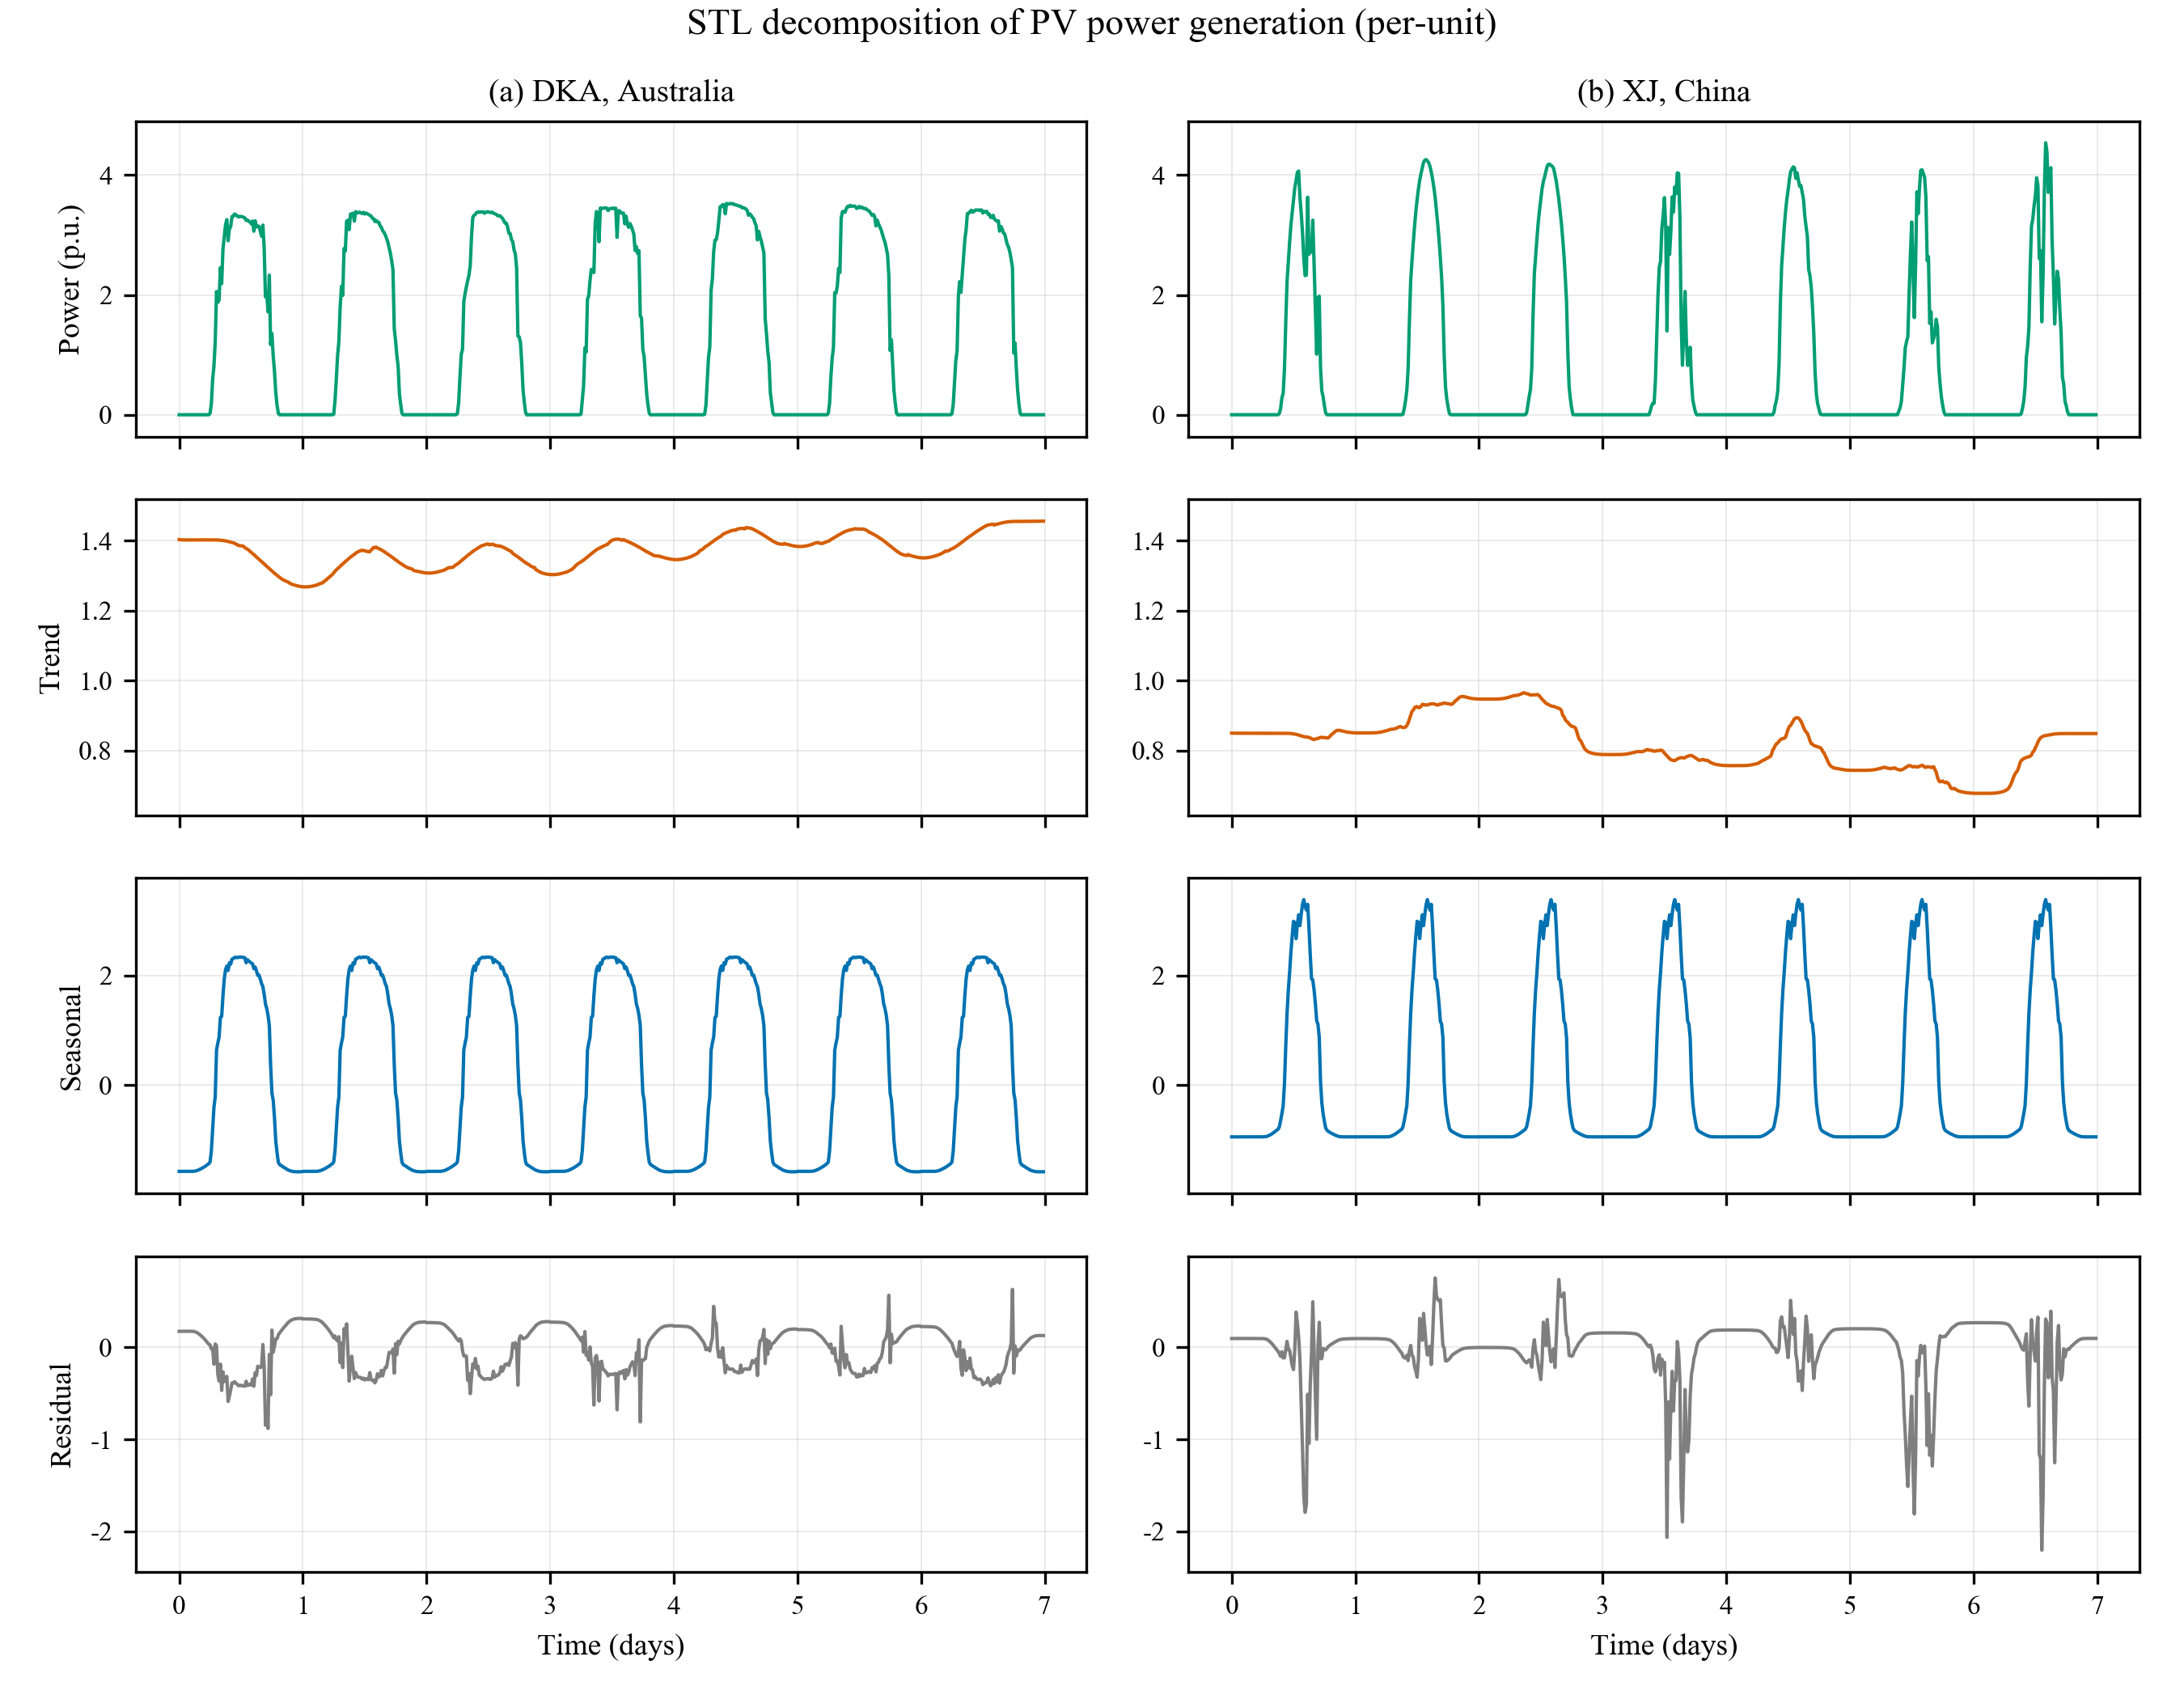
\includegraphics[width=0.85\textwidth]{figures/figA_stl.png}
\caption{STL decomposition of PV power generation in per-unit (left: DKA, Australia; right: XJ, Xinjiang, China)}
\label{fig1}
\end{figure}

\subsection{TimesNet}

The core characteristic of a PV power series is its strong periodicity: the alternation of day and night determines a daily cycle, and the evolution of weather systems superimposes longer cycles on top. How to represent this periodic structure explicitly in a model is the key to the task. TimesNet proposes a representation based on two-dimensional rearrangement for this purpose [25]; its overall structure is shown in Fig. 2.

Its starting point is the representational limitation of a one-dimensional arrangement. At every instant a time series exhibits two kinds of variation: intra-period variation with respect to adjacent instants, and inter-period variation with respect to points of the same phase in different cycles. A one-dimensional arrangement can express only the former explicitly: the adjacency of neighbouring samples is given directly by their indices, whereas the relation between points of the same phase in different cycles is folded into the index spacing and cannot be exploited directly by a local operator [26,27].

The approach of TimesNet is first to rearrange the series into a two-dimensional tensor by period detection so that both kinds of variation gain locality. Given a series  of length  with  variables, the period is first determined from the FFT amplitude spectrum:

\begin{equation}
A = \text{Avg}\Big(\text{Amp}\big(\text{FFT}(X_{1D})\big)\Big)
\end{equation}

\begin{equation}
\{f_1,\ldots,f_k\} = \arg\operatorname{Top}_k(A)
\end{equation}

\begin{equation}
p_i = \frac{T}{f_i}
\end{equation}

where the peak is taken only within  so as to exclude meaningless high-frequency noise. The series is then folded according to the period :

\begin{equation}
X_{2D,i} = \text{Reshape}_{p_i,\,f_i}\big(\text{Padding}(X_{1D})\big)
\end{equation}

After rearrangement, the column direction of the tensor corresponds to adjacent instants and the row direction to points of the same phase differing by one cycle. Intra-period and inter-period variation are thus both converted into local patterns on the two-dimensional tensor and can be extracted simultaneously by the same convolution kernel [28]. TimesNet stacks TimesBlocks in a residual manner, re-estimating the period on the deep features at each layer, and aggregates the convolution results of the  periods with weights obtained by normalising the amplitudes through softmax:

\begin{equation}
X^{l} = \text{TimesBlock}(X^{l-1}) + X^{l-1}
\end{equation}

\begin{equation}
X^{l} = \sum_{i=1}^{k}\hat{A}_{f_i}\cdot\text{Inception}\big(X^{l}_{2D,i}\big)
\end{equation}

where  is the multi-size two-dimensional convolution block.

The effectiveness of the structure above depends on the accuracy of period estimation and the coverage of the convolution kernel [29]; the two improvements that follow target exactly these two points.

\begin{figure}[htbp]
\centering
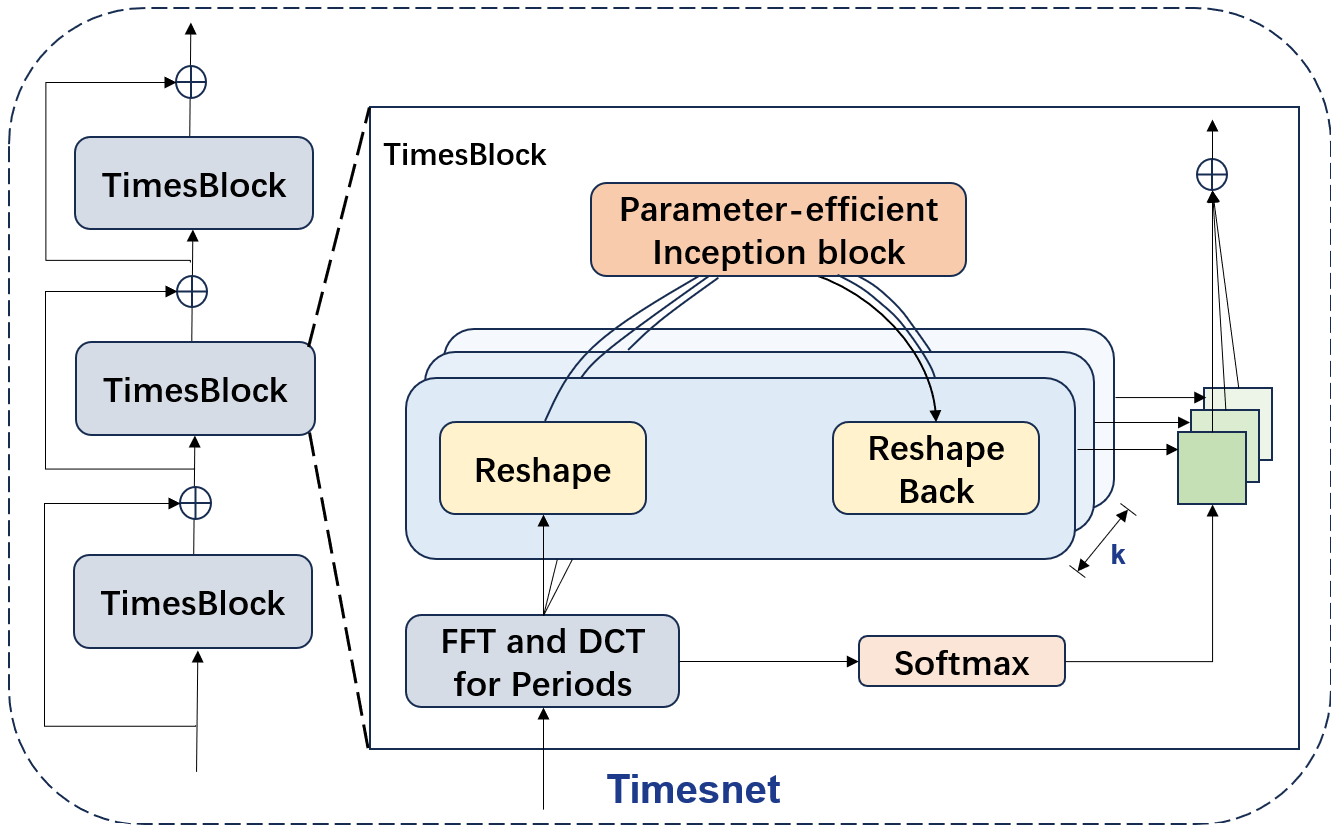
\includegraphics[width=0.85\textwidth]{figures/fig2_timesnet.png}
\caption{Structure of the TimesNet model}
\label{fig2}
\end{figure}

\subsection{Autoformer encoder branch}

TimesNet aggregates inter-period information along the row direction by two-dimensional convolution, but the coverage of the convolution kernel is limited. The largest kernel in the Inception block has size 11, covering only about $\pm$5 cycles on the folded tensor; more distant same-phase dependencies can only be transferred indirectly by stacking layers, and every temporal block re-estimates the period, which shifts the row alignment after folding, so stacking does not reliably widen this range. Enlarging the kernel makes the parameter count grow with the square of the kernel size, while deepening the network is disturbed by the re-estimated period. The convolution branch therefore lacks a scalable way of aggregating same-phase information over long distances. To retain intra-period modelling capability while obtaining long-lag aggregation unrestricted by kernel size, we introduce an Autoformer encoder layer as the second parallel branch [30].

The structure of this encoder layer is shown in Fig. 3, and its core is the auto-correlation mechanism. Unlike self-attention, which assigns weights according to the point-wise similarity of Query and Key, auto-correlation is based on the delay similarity of the series itself [31]. For a real discrete process , the auto-correlation at lag  is defined as

\begin{equation}
\mathcal{R}_{\mathcal{XX}}(\tau) = \lim_{L\to\infty}\frac{1}{L}\sum_{t=1}^{L}\mathcal{X}_t\,\mathcal{X}_{t-\tau}
\end{equation}

It describes the degree of similarity between the series and its version lagged by  steps. The rationale is that sub-processes at the same phase position in different cycles are naturally similar, so  takes significant values when  is an integer multiple of the period and can be regarded as an unnormalised confidence of the period length . A direct computation by definition costs , which the Wiener--Khinchin theorem reduces to :

\begin{equation}
\mathcal{S}_{\mathcal{XX}}(f) = \mathcal{F}(\mathcal{X}_t)\,\overline{\mathcal{F}(\mathcal{X}_t)}
\end{equation}

\begin{equation}
\mathcal{R}_{\mathcal{XX}}(\tau) = \mathcal{F}^{-1}\big(\mathcal{S}_{\mathcal{XX}}(f)\big)
\end{equation}

Let  be linearly projected to obtain ,  and . The mechanism first selects the k delays with the highest confidence and then, using their normalised confidences as weights, performs time-delay aggregation of the Value at each delay:

\begin{equation}
\tau_1,\ldots,\tau_k = \arg\underset{\tau\in\{1,\ldots,L\}}{\operatorname{Top}_k}\big(\mathcal{R}_{\mathcal{QK}}(\tau)\big)
\end{equation}

\begin{equation}
\hat{\mathcal{R}}_{\mathcal{QK}}(\tau_1),\ldots,\hat{\mathcal{R}}_{\mathcal{QK}}(\tau_k) = \text{Softmax}\big(\mathcal{R}_{\mathcal{QK}}(\tau_1),\ldots,\mathcal{R}_{\mathcal{QK}}(\tau_k)\big)
\end{equation}

\begin{equation}
\text{AutoCorrelation}(\mathcal{Q},\mathcal{K},\mathcal{V}) = \sum_{i=1}^{k}\text{Roll}(\mathcal{V},\tau_i)\,\hat{\mathcal{R}}_{\mathcal{QK}}(\tau_i)
\end{equation}

where  shifts  by  steps along the time axis and  with c a hyper-parameter. This aggregation differs fundamentally from the point-wise weighting of self-attention: it aligns as a whole the similar sub-sequences at the same phase and then sums them with weights, so when the delay happens to be the true period, what is aggregated is precisely the same-phase points separated by an integer number of cycles. Information can therefore cross arbitrarily long lags in a single operation, without the layer-by-layer accumulation required by convolution, and the gap left by the structure described above is thereby filled.

The original Autoformer encoder applies a series decomposition after each sub-layer in order to separate and discard the trend component [32]. In this paper the decomposition is already performed by the STL module at the input, so to avoid two decomposition mechanisms within one model it is not repeated here; only the auto-correlation sub-layer and the feed-forward network are retained, each with a residual connection and layer normalisation:

\begin{equation}
Z = \text{LayerNorm}\big(X + \text{AutoCorrelation}(X)\big)
\end{equation}

\begin{equation}
H = \text{LayerNorm}\big(Z + \text{FFN}(Z)\big)
\end{equation}

where the feed-forward network is a two-layer fully connected structure.

\begin{figure}[htbp]
\centering
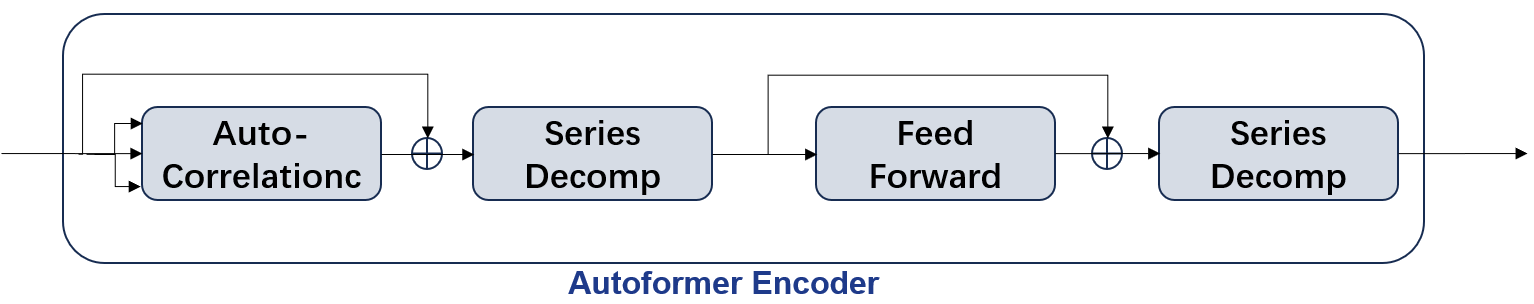
\includegraphics[width=0.85\textwidth]{figures/fig3_autoformer_enc.png}
\caption{Structure of the Autoformer encoder layer}
\label{fig3}
\end{figure}

\subsection{FFT-DCT dual-domain period detection}

The accuracy of period estimation directly determines whether the two-dimensional structure holds, so period detection needs to be examined separately.

TimesNet determines the period from the peak of the FFT amplitude spectrum. For a series of length , the FFT is

\begin{equation}
\hat{X}[j] = \sum_{t=0}^{T-1} X[t]\,e^{-2\pi ijt/T}
\end{equation}

Because the spectrum takes values only at the discrete frequencies , the detectable periods are restricted to

\begin{equation}
\mathcal{P}_{\text{FFT}} = \left\{\frac{T}{j}\ \middle|\ j = 1,\ldots,\left\lfloor \tfrac{T}{2}\right\rfloor\right\}
\end{equation}

this set of grid points. When the true period  does not fall on a grid point, a deviation exists between the detected  and , and this deviation makes the rows of the two-dimensional tensor shift one by one and weakens inter-period locality. The grid is particularly sparse at long periods: the spacing between adjacent points is about , so the resolution falls as the period grows.

To remedy this, a second set of period grids is introduced. DCT-II uses a cosine basis with a half-sample offset:

\begin{equation}
\tilde{X}[k] = \sum_{t=0}^{T-1} X[t]\,\cos\!\left(\frac{\pi k(2t+1)}{2T}\right)
\end{equation}

Compared with FFT, the frequency index differs by a factor of two: the  -th basis contains only  complete cycles within the window, so the detectable periods are . Expanding by the parity of  gives: when  is even,  coincides with the FFT grid; when  is odd, it gives , which lies midway between adjacent FFT grid points. The DCT grid is therefore a refinement of the FFT grid: it retains every period representable by FFT and additionally provides candidates at half-interval positions. If the true period falls between two FFT grid points, DCT may yield an estimate closer to , thereby improving row alignment.

Accordingly, two detection paths are run in parallel on the same input: the FFT path takes the Top-K periods, and the DCT path applies DCT-II and likewise takes the Top-K peaks. Each path performs folding and convolution with its own set of periods, the parameters are not shared, and the outputs are concatenated along the feature dimension and fused by a fully connected layer.

A refined grid is valuable only if the additional candidates really are true periods; if they merely correspond to noise peaks in the amplitude spectrum, their folded rows do not form a same-phase relation and instead introduce noise. This paper therefore does not presuppose that DCT brings a gain, but treats it as a testable hypothesis to be decided by ablation.

\subsection{PA-STL-DualTimesNet model}

The overall structure of the proposed parallel STL dual-domain TimesNet (PA-STL-DualTimesNet) is shown in Fig. 4 and consists of the following parts. First, STL decomposes PV power into trend, seasonal and residual components, and the three components are mapped by embedding networks with independent parameters and then added to form the reconstructed input features. The backbone is then formed by stacking N dual-domain temporal blocks (N is 2 by default).

Two branches are set in parallel within each block: the dual-domain periodic convolution branch extracts intra-period and near-neighbour inter-period variation by period folding and two-dimensional convolution, while the Autoformer encoder branch selects delays from the correlation spectrum and aggregates same-phase points over arbitrarily long lags along the original time axis. The outputs of the two branches are concatenated along the feature dimension, passed through a fully connected layer to map back to the original dimension, added to the input residual and normalised:

\begin{equation}
H = \text{LayerNorm}\Big(x + \mathbf{W}_f\big[\text{Conv}(x);\text{AutoCorr}(x)\big] + \mathbf{b}_f\Big)
\end{equation}

where  and  are the weight matrix and bias of this fully connected layer, respectively.

Parallel rather than serial composition is adopted because the two branches require different inputs: the encoder branch depends on the lag semantics of the original time axis, whereas two-dimensional folding is a rearrangement that destroys those semantics, so if it followed the convolution branch the resulting  would no longer correspond to a real time delay; conversely, the convolution branch depends on the phase alignment produced by folding, which would likewise be destroyed if it followed auto-correlation. Each branch starting directly from the same hidden representation allows the two kinds of inter-period aggregation to be carried out in their own meaningful coordinate systems. Their failure conditions also differ: the convolution branch is affected by period-estimation error, whereas the encoder branch is affected by the quality of the correlation spectrum; parallel composition lets the model fall back on one when the other is unreliable, which is why the fusion weights are left to be learned by the network itself.

It should be noted that ``parallel'' here means that both branches take the same hidden representation as input and are not data-dependent on each other. This is not on the same level as the parallel computation represented by Informer (which describes whether the computation can be parallelised) or the multi-period parallelism represented by TimesNet (which describes multi-scale processing).

Finally, the output of the backbone is projected into the forecasting space by a fully connected layer and denormalised to give the final power forecast.

\begin{figure}[htbp]
\centering
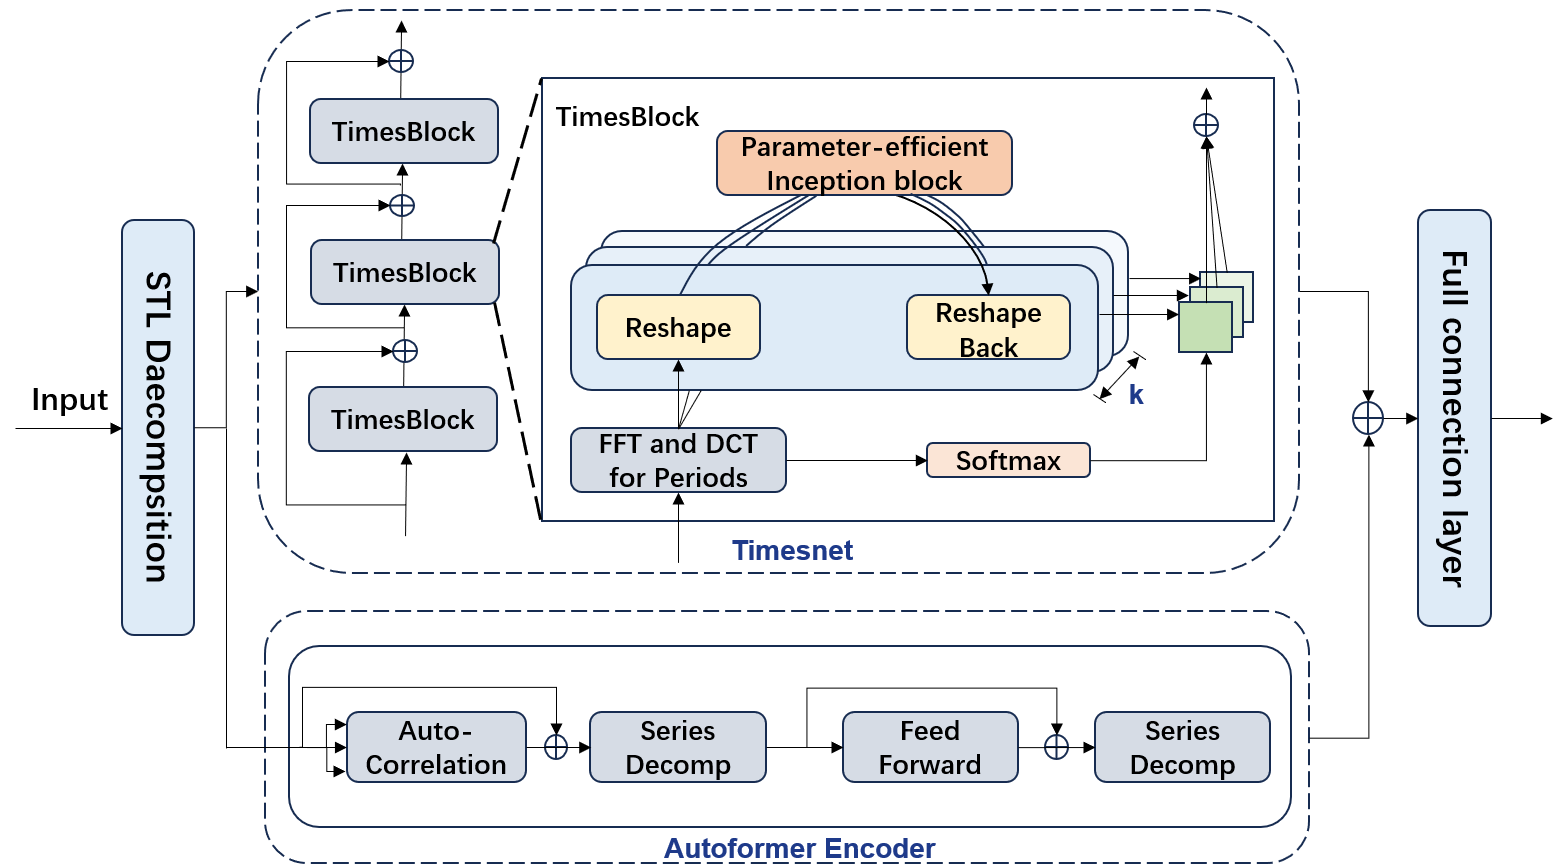
\includegraphics[width=0.85\textwidth]{figures/fig4_architecture.png}
\caption{Architecture of PA-STL-DualTimesNet}
\label{fig4}
\end{figure}

\section{DATA AND EXPERIMENTAL SETUP}

\subsection{Data description}

Two real PV datasets are used to evaluate the model. They come from Australia and China respectively and differ markedly in climate and volatility, which provides a natural contrast for testing the model under different conditions.

The first dataset comes from the DKA Solar Centre in Darwin, Northern Territory, Australia (denoted Solar-DKA). The centre publishes measured data for several PV arrays, of which the multivariate power and meteorological records are used here. The sampling interval is 5 minutes, the time span is January 2014 to November 2015, and there are 192,375 records in total. The data contain 10 numerical variables: the generated power Active\_Power (the forecasting target) and nine meteorological variables --- wind speed, air temperature, relative humidity, global horizontal radiation, diffuse horizontal radiation, wind direction, daily rainfall, global tilted radiation and diffuse tilted radiation. The area has a tropical monsoon climate with high temperatures and abundant sunshine throughout the year, and the generated power is relatively stable overall.

The second dataset comes from a PV plant in the Xinjiang Uygur Autonomous Region of China (denoted Solar-XJ). The sampling interval is 15 minutes, the time span is the whole of 2023, and there are 35,040 records with no missing values. The data contain 8 numerical variables: the actual generated power (the forecasting target) and seven meteorological variables --- module temperature, ambient temperature, pressure, humidity, global radiation, direct radiation and diffuse radiation. The area has a temperate continental climate with a large diurnal temperature range and frequent weather changes.

Compared with the first dataset, the second has a markedly higher proportion of days with pronounced power fluctuation. This difference is precisely the motivation for the season- and volatility-grouped experiments: if the relative gain of the model is larger under volatile conditions, its improvement indeed comes from more robust modelling of the periodic structure and the long-lag dependence, rather than being effective only under stable conditions. Table 1 gives the detailed characteristics of the two datasets.

\begin{table}[htbp]
\caption{Table 1  Description of the datasets}
\centering
\begin{tabular}{l c c}
\hline
Item & Solar-DKA (Australia) & Solar-XJ (Xinjiang, China) \\
\hline
Sampling interval & 5 min & 15 min \\
Time span & Jan 2014 - Nov 2015 (about 2 years) & Jan 2023 - Dec 2023 (1 year) \\
Number of samples & 192,375 & 35,040 \\
Number of variables & 10 & 8 \\
Dominant variable & Global horizontal irradiance & Global irradiance \\
Climate type & Tropical monsoon & Temperate continental \\
Volatility & Lower & Higher \\
\hline
\end{tabular}
\label{tab1}
\end{table}

\subsection{Data preprocessing}

To make the two datasets comparable, the 5-minute Solar-DKA data are first resampled to 15 minutes, so that both have the same sampling interval and a daily cycle of 96 samples, eliminating any bias caused by the difference in sampling frequency.

For data cleaning, PV power is physically non-negative and should not exceed the installed capacity; the 3$\sigma$ rule is therefore used to identify outliers, which are set to missing. Short gaps are filled by linear interpolation, and intervals with missing data longer than 3 hours are removed entirely --- such intervals usually correspond to equipment downtime, are hard to impute reliably, and forcing a fill would introduce spurious periodic structure.

For the features, the maximal information coefficient (MIC) is used to measure the correlation between each meteorological variable and the generated power. MIC captures both linear and nonlinear dependence and is suitable for a complex relationship such as irradiance versus power. The results are shown in Fig. 5: in both datasets the irradiance variables (global, direct and diffuse radiation) have MIC values clearly higher than the others and are the dominant inputs; module temperature shows a moderate correlation; and pressure, wind direction and rainfall have the lowest MIC. Variables with MIC below 0.1 are therefore removed to reduce the input dimension and the risk of overfitting. Comparing the two datasets, the correlations among variables are generally higher in the Xinjiang data, indicating that the power at this site is more strongly affected by several factors jointly and that a single variable has weaker explanatory power.

\begin{figure}[htbp]
\centering
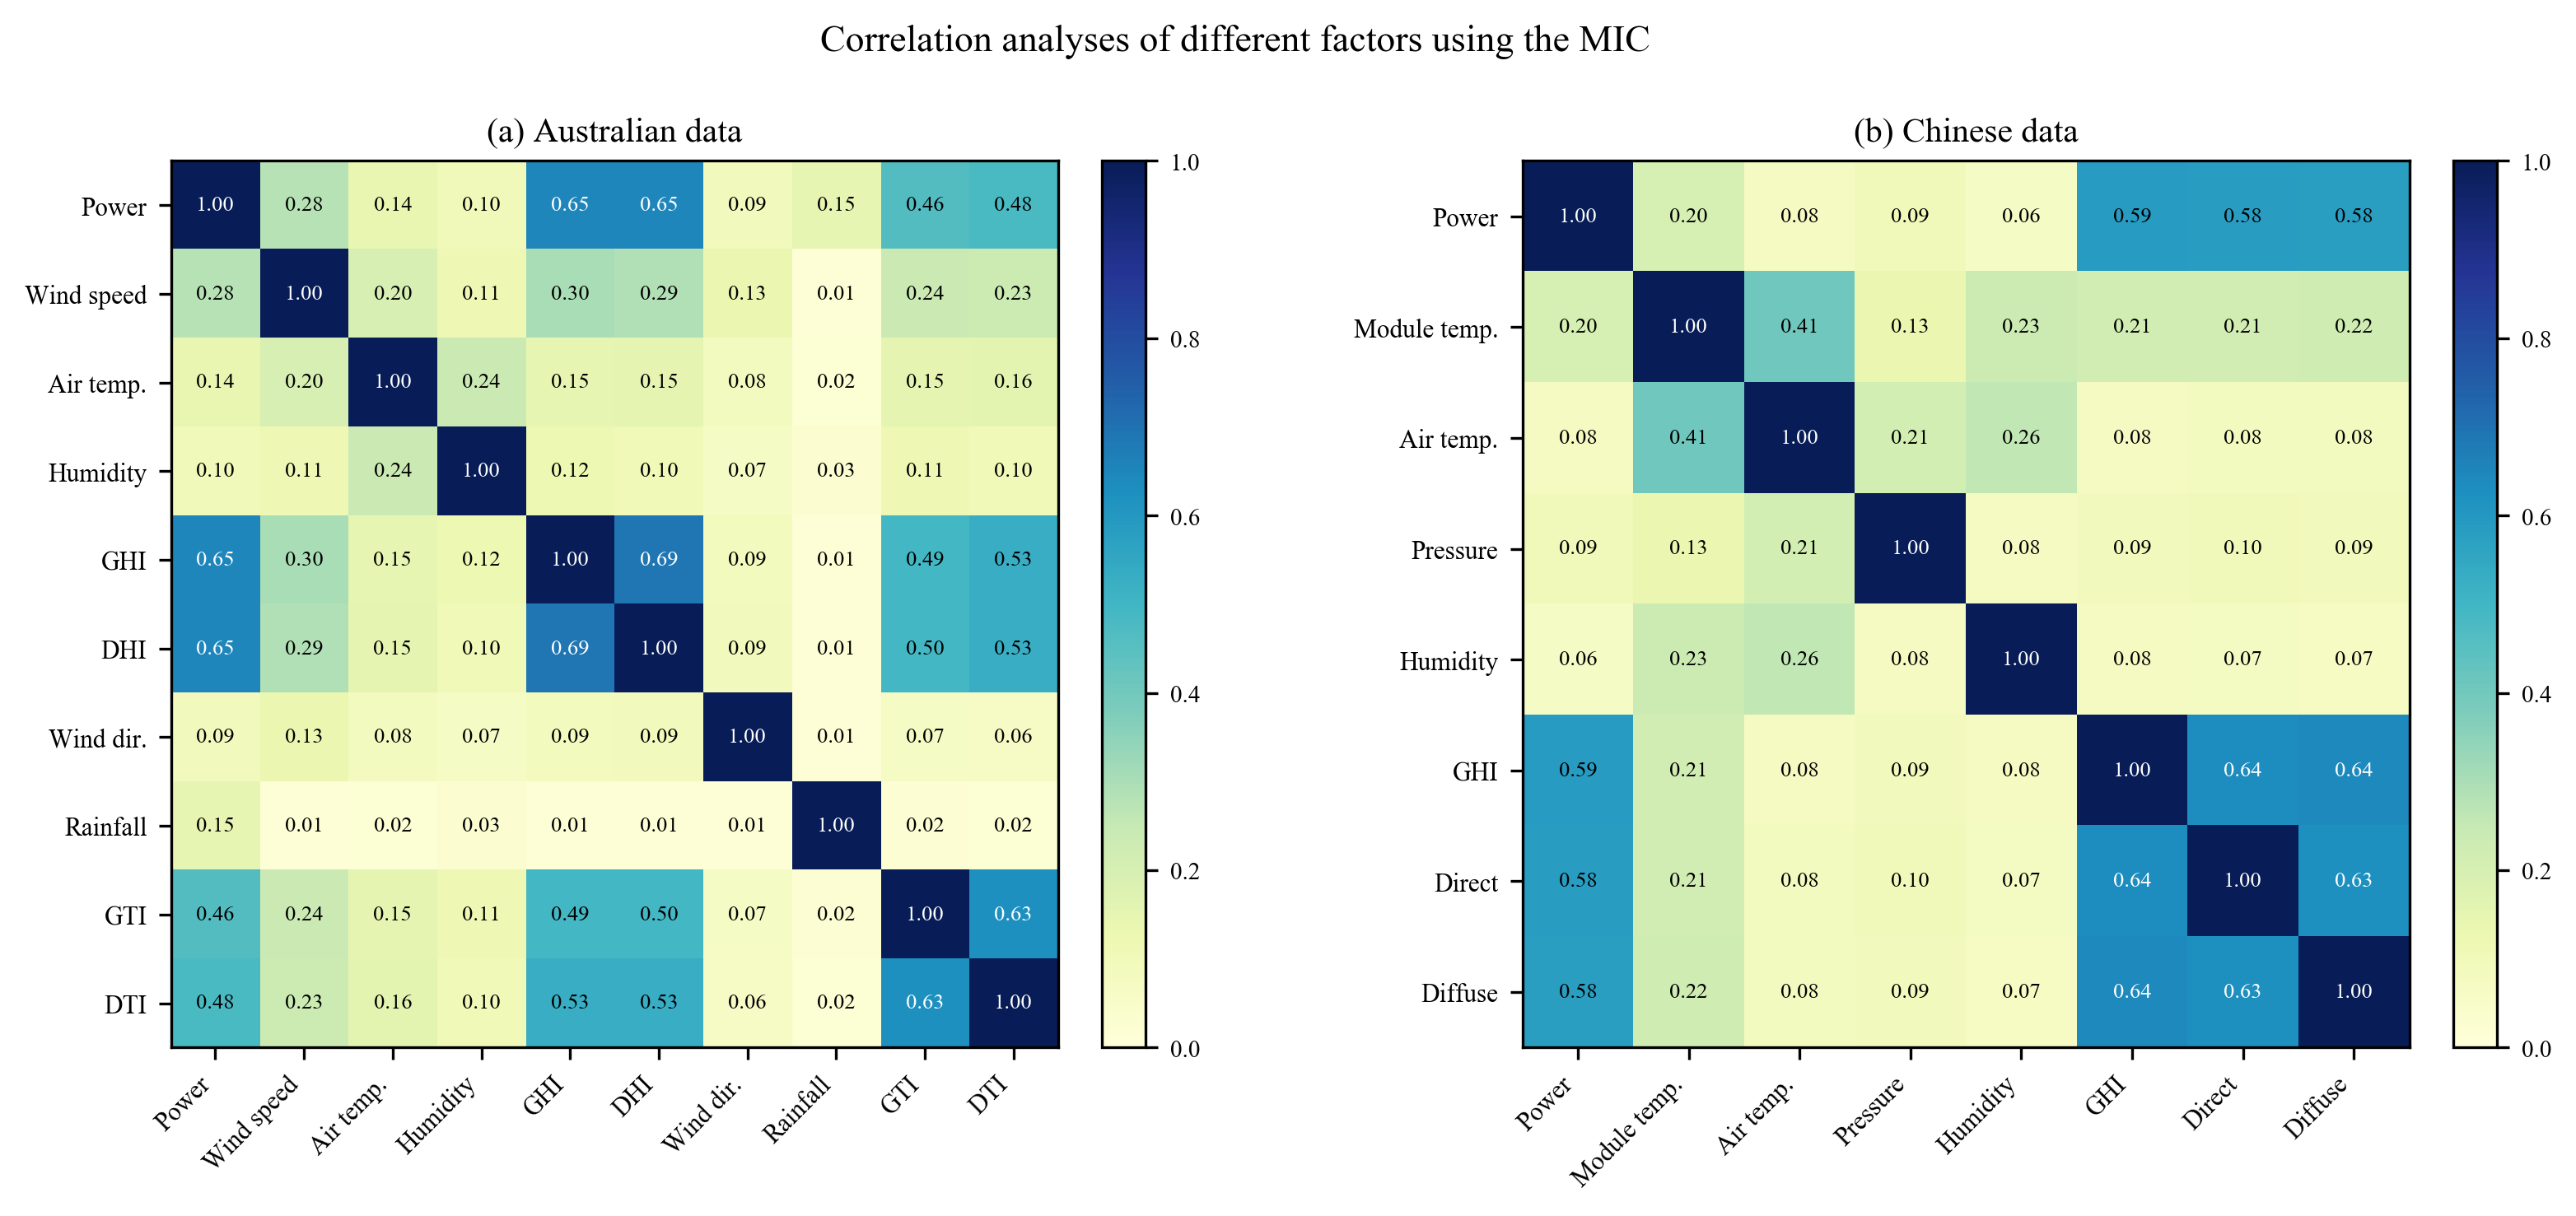
\includegraphics[width=0.85\textwidth]{figures/figB_mic.png}
\caption{Correlation analyses of different factors using the MIC: (a) Australian data; (b) Chinese data}
\label{fig5}
\end{figure}

Finally, the power and meteorological variables are normalised to zero mean and unit variance, with the statistics fitted on the training set only and then applied to the validation and test sets; the data are split chronologically into training, validation and test sets in a 6:2:2 ratio without shuffling, so as to avoid future-information leakage. The validation set is used for early stopping and model selection, and the test set only for final evaluation. The datasets retain all periods and no daytime filtering is applied. Night-time power is constantly zero, which does dilute the error signal during the day, but filtering the night would make ``one day'' no longer 96 samples and destroy the correspondence between the daily cycle and the number of steps. To avoid the effect of the night-time zeros, the evaluation also reports R$^2$ and MASE, which are not affected by zeros, in addition to RMSE and MAE.

The STL decomposition period is taken as one daily cycle, i.e. p = 96 steps; the constraint T $\geq$ 2p requires the input length to be no less than 192 steps.

\subsection{Baseline models}

To evaluate the performance of the proposed model, eight models are selected for comparison, covering four families of methods: machine learning, recurrent networks, linear models and Transformers.

The machine-learning methods are K-nearest neighbours (KNN) and LightGBM; both are simple to construct and fast to train and serve as a reference for assessing the need for deep models. The recurrent networks are LSTM and BiLSTM, the former a classical method of time-series modelling and the latter aggregating context in both directions. DLinear consists of a linear decomposition plus a multilayer perceptron and is a widely cited simple strong baseline used to test the need for complex structures. PatchTST splits the series into patches and models them with a Transformer, representing the patch-based approach. Autoformer introduces the auto-correlation mechanism and series decomposition and is the source of this paper's encoder branch; including it in the comparison shows directly the difference between ``borrowing its component'' and ``using the model as it is''. TimesNet is the model this paper improves directly and is the main baseline.

All baselines are trained and evaluated under the same data split, the same input and output lengths and the same normalisation procedure, so that the comparison is fair. The hyper-parameter configuration of the proposed model is given in Table 2.

\begin{table}[htbp]
\caption{Table 2  Hyperparameter configuration}
\centering
\begin{tabular}{l c}
\hline
Parameter & Value \\
\hline
Hidden dimension d\_model & 64 \\
Feed-forward dimension d\_ff & 64 \\
Backbone layers e\_layers & 2 \\
Inception branches num\_kernels & 6 \\
Top-K periods & 5 \\
Decomposition period p & 96 (both datasets) \\
Batch size & 32 \\
Optimizer & Adam \\
Initial learning rate & 1e-3 \\
Learning-rate schedule & Halved every epoch \\
Early-stopping patience & 3 \\
\hline
\end{tabular}
\label{tab2}
\end{table}

The loss during training is shown in Fig. 6. The training and validation losses fall rapidly in the first few epochs and then level off; the validation loss reaches its minimum in the middle of training and does not improve afterwards, at which point early stopping terminates training. The gap between the two curves is small and no obvious overfitting occurs.

\begin{figure}[htbp]
\centering
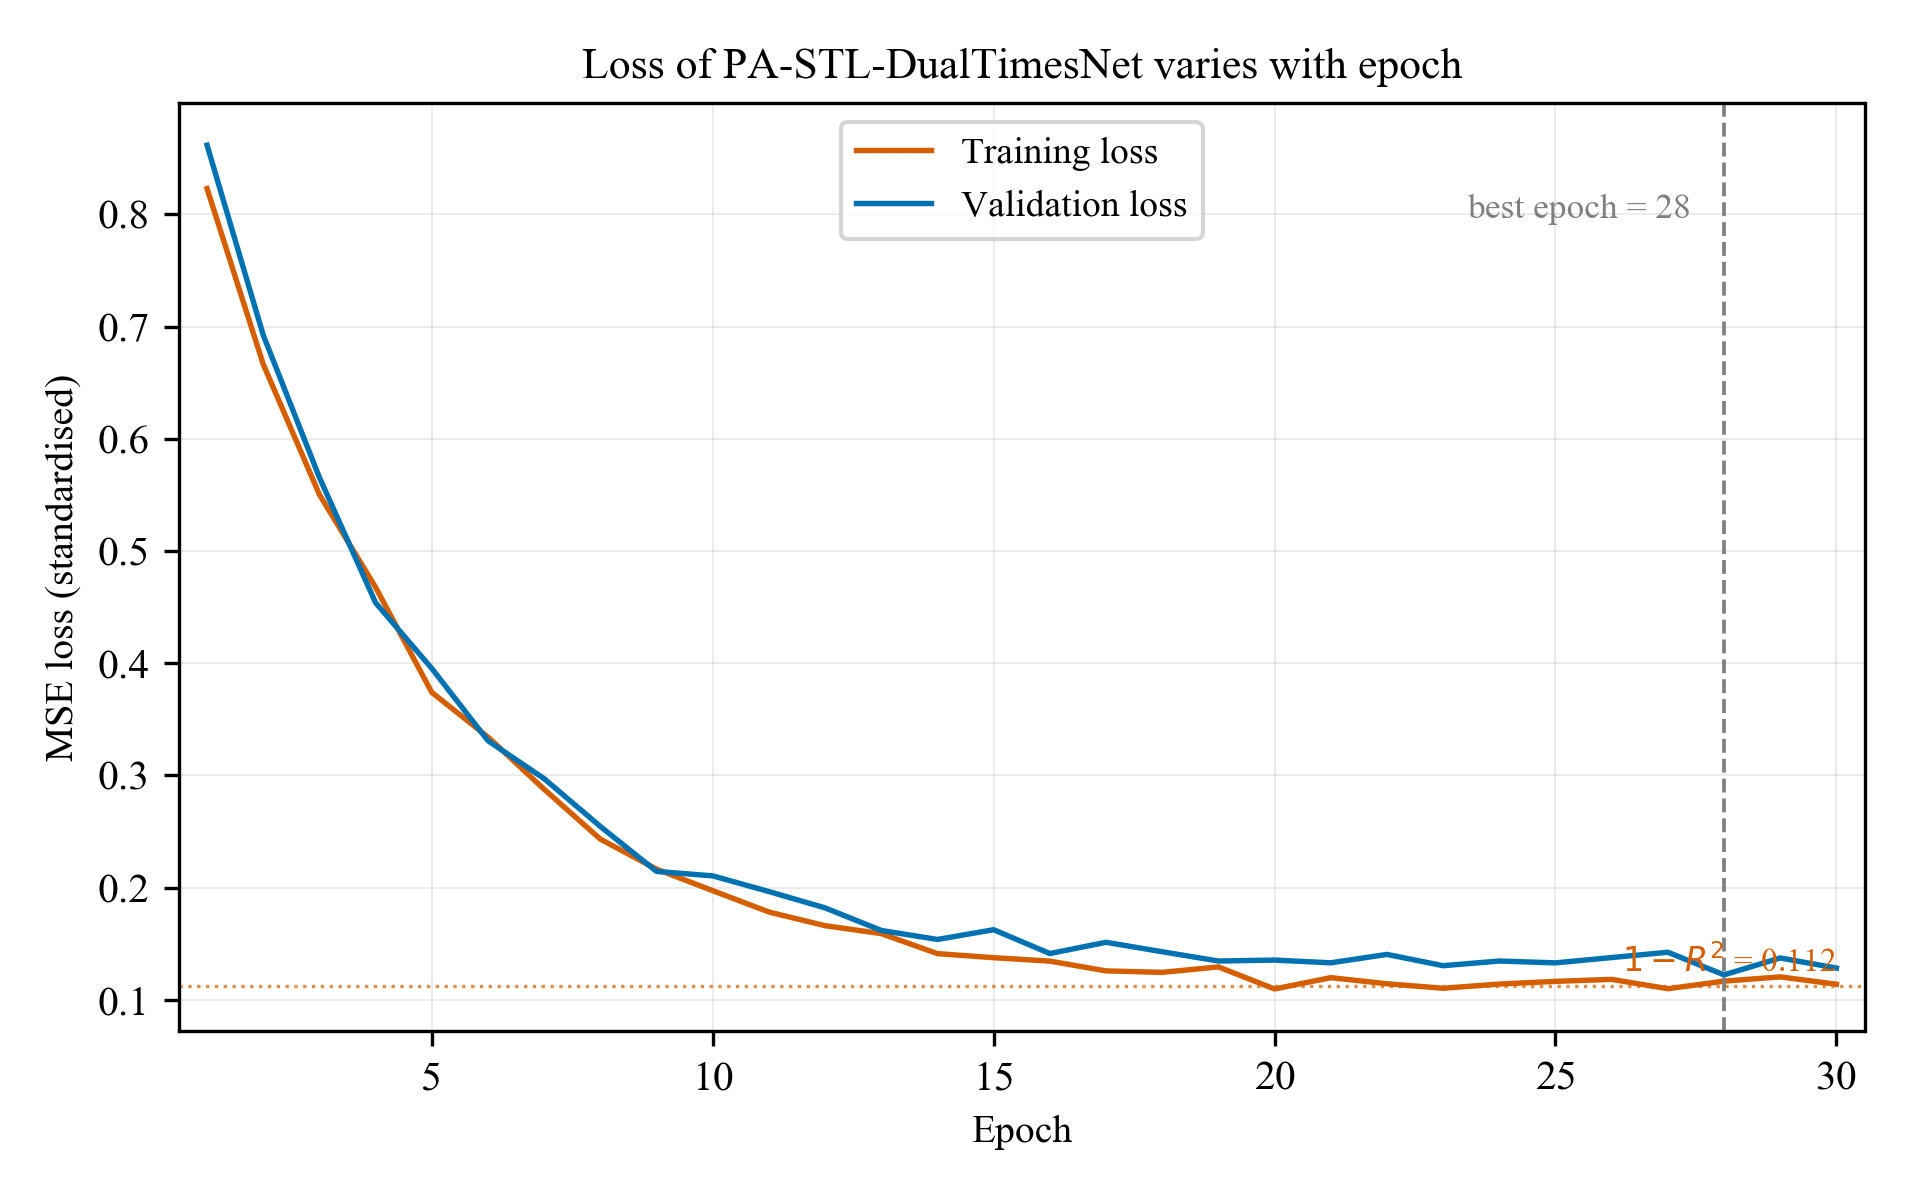
\includegraphics[width=0.85\textwidth]{figures/fig8_loss.png}
\caption{Loss of PA-STL-DualTimesNet varies with epoch}
\label{fig6}
\end{figure}

\subsection{Evaluation metrics}

To evaluate the model on the test set, four metrics are adopted --- mean absolute error (MAE), root mean square error (RMSE), mean absolute scaled error (MASE) and the coefficient of determination (R$^2$) --- defined as follows:

\begin{equation}
\text{MAE} = \frac{1}{N}\sum_{i=1}^{N}|y_i - \hat{y}_i|
\end{equation}

\begin{equation}
\text{RMSE} = \sqrt{\frac{1}{N}\sum_{i=1}^{N}(y_i-\hat{y}_i)^2}
\end{equation}

\begin{equation}
\text{MASE} = \frac{1}{N}\sum_{i=1}^{N}\frac{|y_i-\hat{y}_i|}{\frac{1}{N-96}\sum_{j=97}^{N}|y_j-y_{j-96}|}
\end{equation}

\begin{equation}
R^2 = 1 - \frac{\sum_{i=1}^{N}(y_i-\hat{y}_i)^2}{\sum_{i=1}^{N}(y_i-\bar{y})^2}
\end{equation}

where  and  are the true and predicted values respectively,  is the number of samples and  the mean of the true values. The denominator of MASE is the mean absolute error of the seasonal naive forecast (one daily cycle apart); a value below 1 means better than this baseline and above 1 worse.

\section{RESULTS AND DISCUSSION}

\subsection{Comparison with different models}

The PA-STL-DualTimesNet model is compared with the baselines described above; the results for the two datasets are given in Table 3 and Table 4.

\begin{table}[htbp]
\caption{Table 3  Comparison with different models (Solar-DKA)}
\centering
\begin{tabular}{l c c c c}
\hline
Model & MAE & RMSE & MASE & R$^2$ \\
\hline
KNN & 153 & 196 & 1.058 & 0.9616 \\
LightGBM & 134 & 172 & 0.927 & 0.9704 \\
LSTM & 125 & 160 & 0.864 & 0.9744 \\
BiLSTM & 123 & 158 & 0.851 & 0.975 \\
DLinear & 112 & 143 & 0.775 & 0.9796 \\
PatchTST & 107 & 136 & 0.74 & 0.9815 \\
Autoformer & 109 & 140 & 0.754 & 0.9804 \\
TimesNet & 101 & 130 & 0.698 & 0.9831 \\
PA-STL-DualTimesNet & 93 & 119 & 0.643 & 0.9858 \\
\hline
\end{tabular}
\label{tab3}
\end{table}

\begin{table}[htbp]
\caption{Table 4  Comparison with different models (Solar-XJ)}
\centering
\begin{tabular}{l c c c c}
\hline
Model & MAE & RMSE & MASE & R$^2$ \\
\hline
KNN & 142 & 182 & 0.784 & 0.9669 \\
LightGBM & 126 & 161 & 0.695 & 0.9741 \\
LSTM & 114 & 146 & 0.629 & 0.9787 \\
BiLSTM & 112 & 144 & 0.618 & 0.9793 \\
DLinear & 102 & 131 & 0.563 & 0.9828 \\
PatchTST & 98 & 126 & 0.541 & 0.9841 \\
Autoformer & 100 & 129 & 0.552 & 0.9834 \\
TimesNet & 96 & 123 & 0.53 & 0.9849 \\
PA-STL-DualTimesNet & 88 & 113 & 0.486 & 0.9872 \\
\hline
\end{tabular}
\label{tab4}
\end{table}

The comparison shows that machine-learning models are limited in their ability to capture temporal dependence and have clearly higher errors than the deep models; recurrent networks outperform the machine-learning models but still model long lags inadequately; DLinear reaches a level close to the deep models with a very simple structure, which shows that the baselines themselves are strong; PatchTST and Autoformer perform similarly, and the latter --- the source of this paper's encoder branch --- is less accurate than the proposed model, which shows that decoupling the auto-correlation sub-layer from the complete model and combining it in parallel with the period-folding path is effective. The proposed model outperforms all baselines on the four metrics, and the conclusion is consistent across the two datasets.

Fig. 7 shows the MAE of each model as a bar chart. The ranking of the models is exactly the same for the two datasets, the proposed model being lowest in both, which agrees with the conclusions of Tables 3 and 4 and shows that the advantage is not incidental.

\begin{figure}[htbp]
\centering
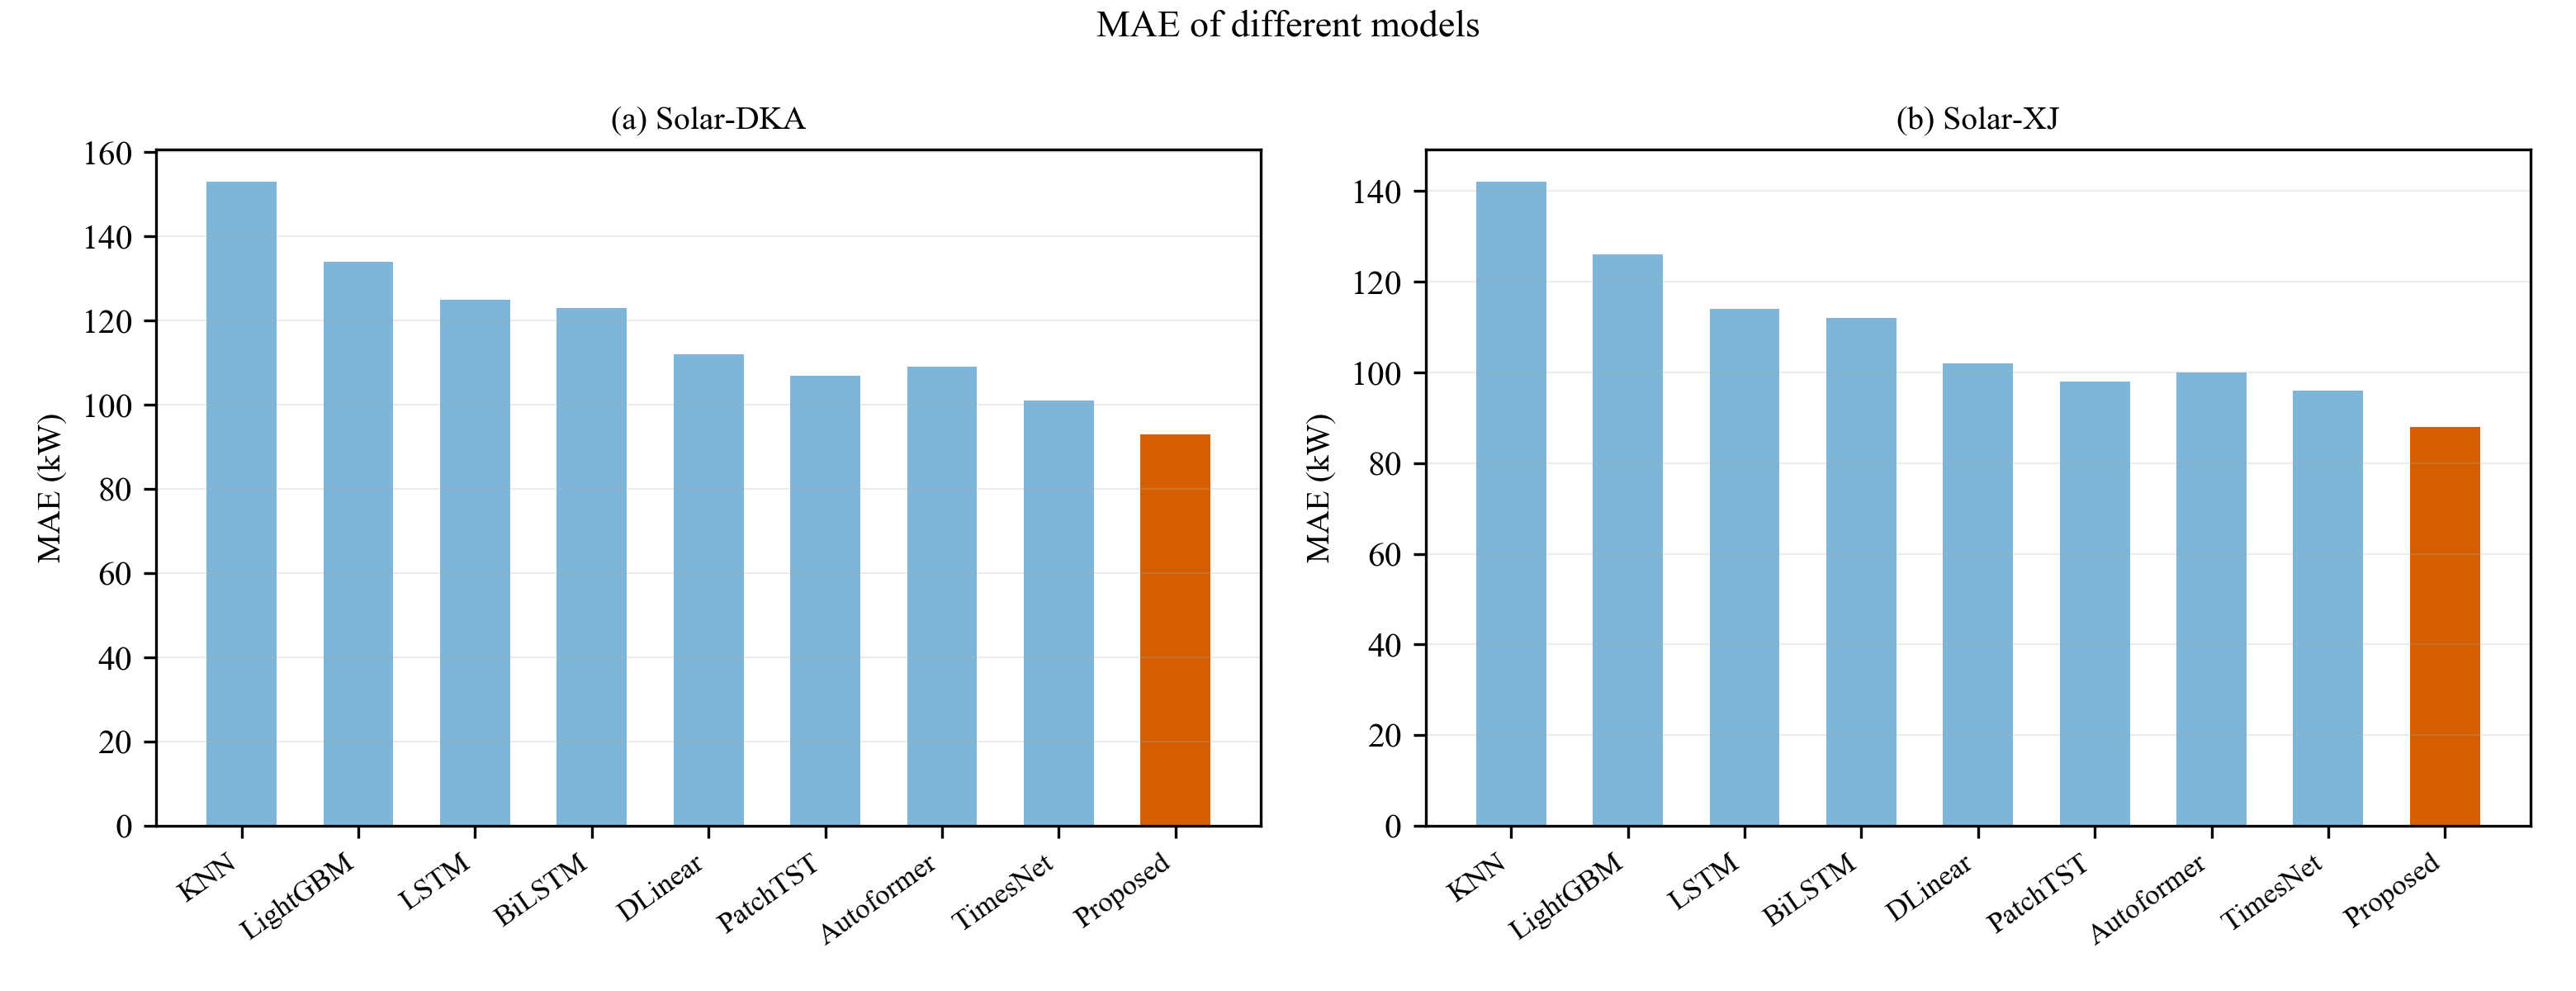
\includegraphics[width=0.85\textwidth]{figures/fig5_model_bars.png}
\caption{MAE of different models}
\label{fig7}
\end{figure}

An overall error can only reflect average performance, so Fig. 8 gives the prediction curves on some test samples (four days, 384 sampling points in total). All models capture the daily waveform of the true power, and the differences are concentrated in the periods of rapid power ramping: there the baselines deviate noticeably more, while the proposed model tracks the true values most closely. Fig. 9 gives the same judgement from the point-by-point perspective. The scatter of the proposed model lies closer to the diagonal; in the high-power region the baselines generally underestimate the peak power, whereas the proposed model has a smaller deviation.

\begin{figure}[htbp]
\centering
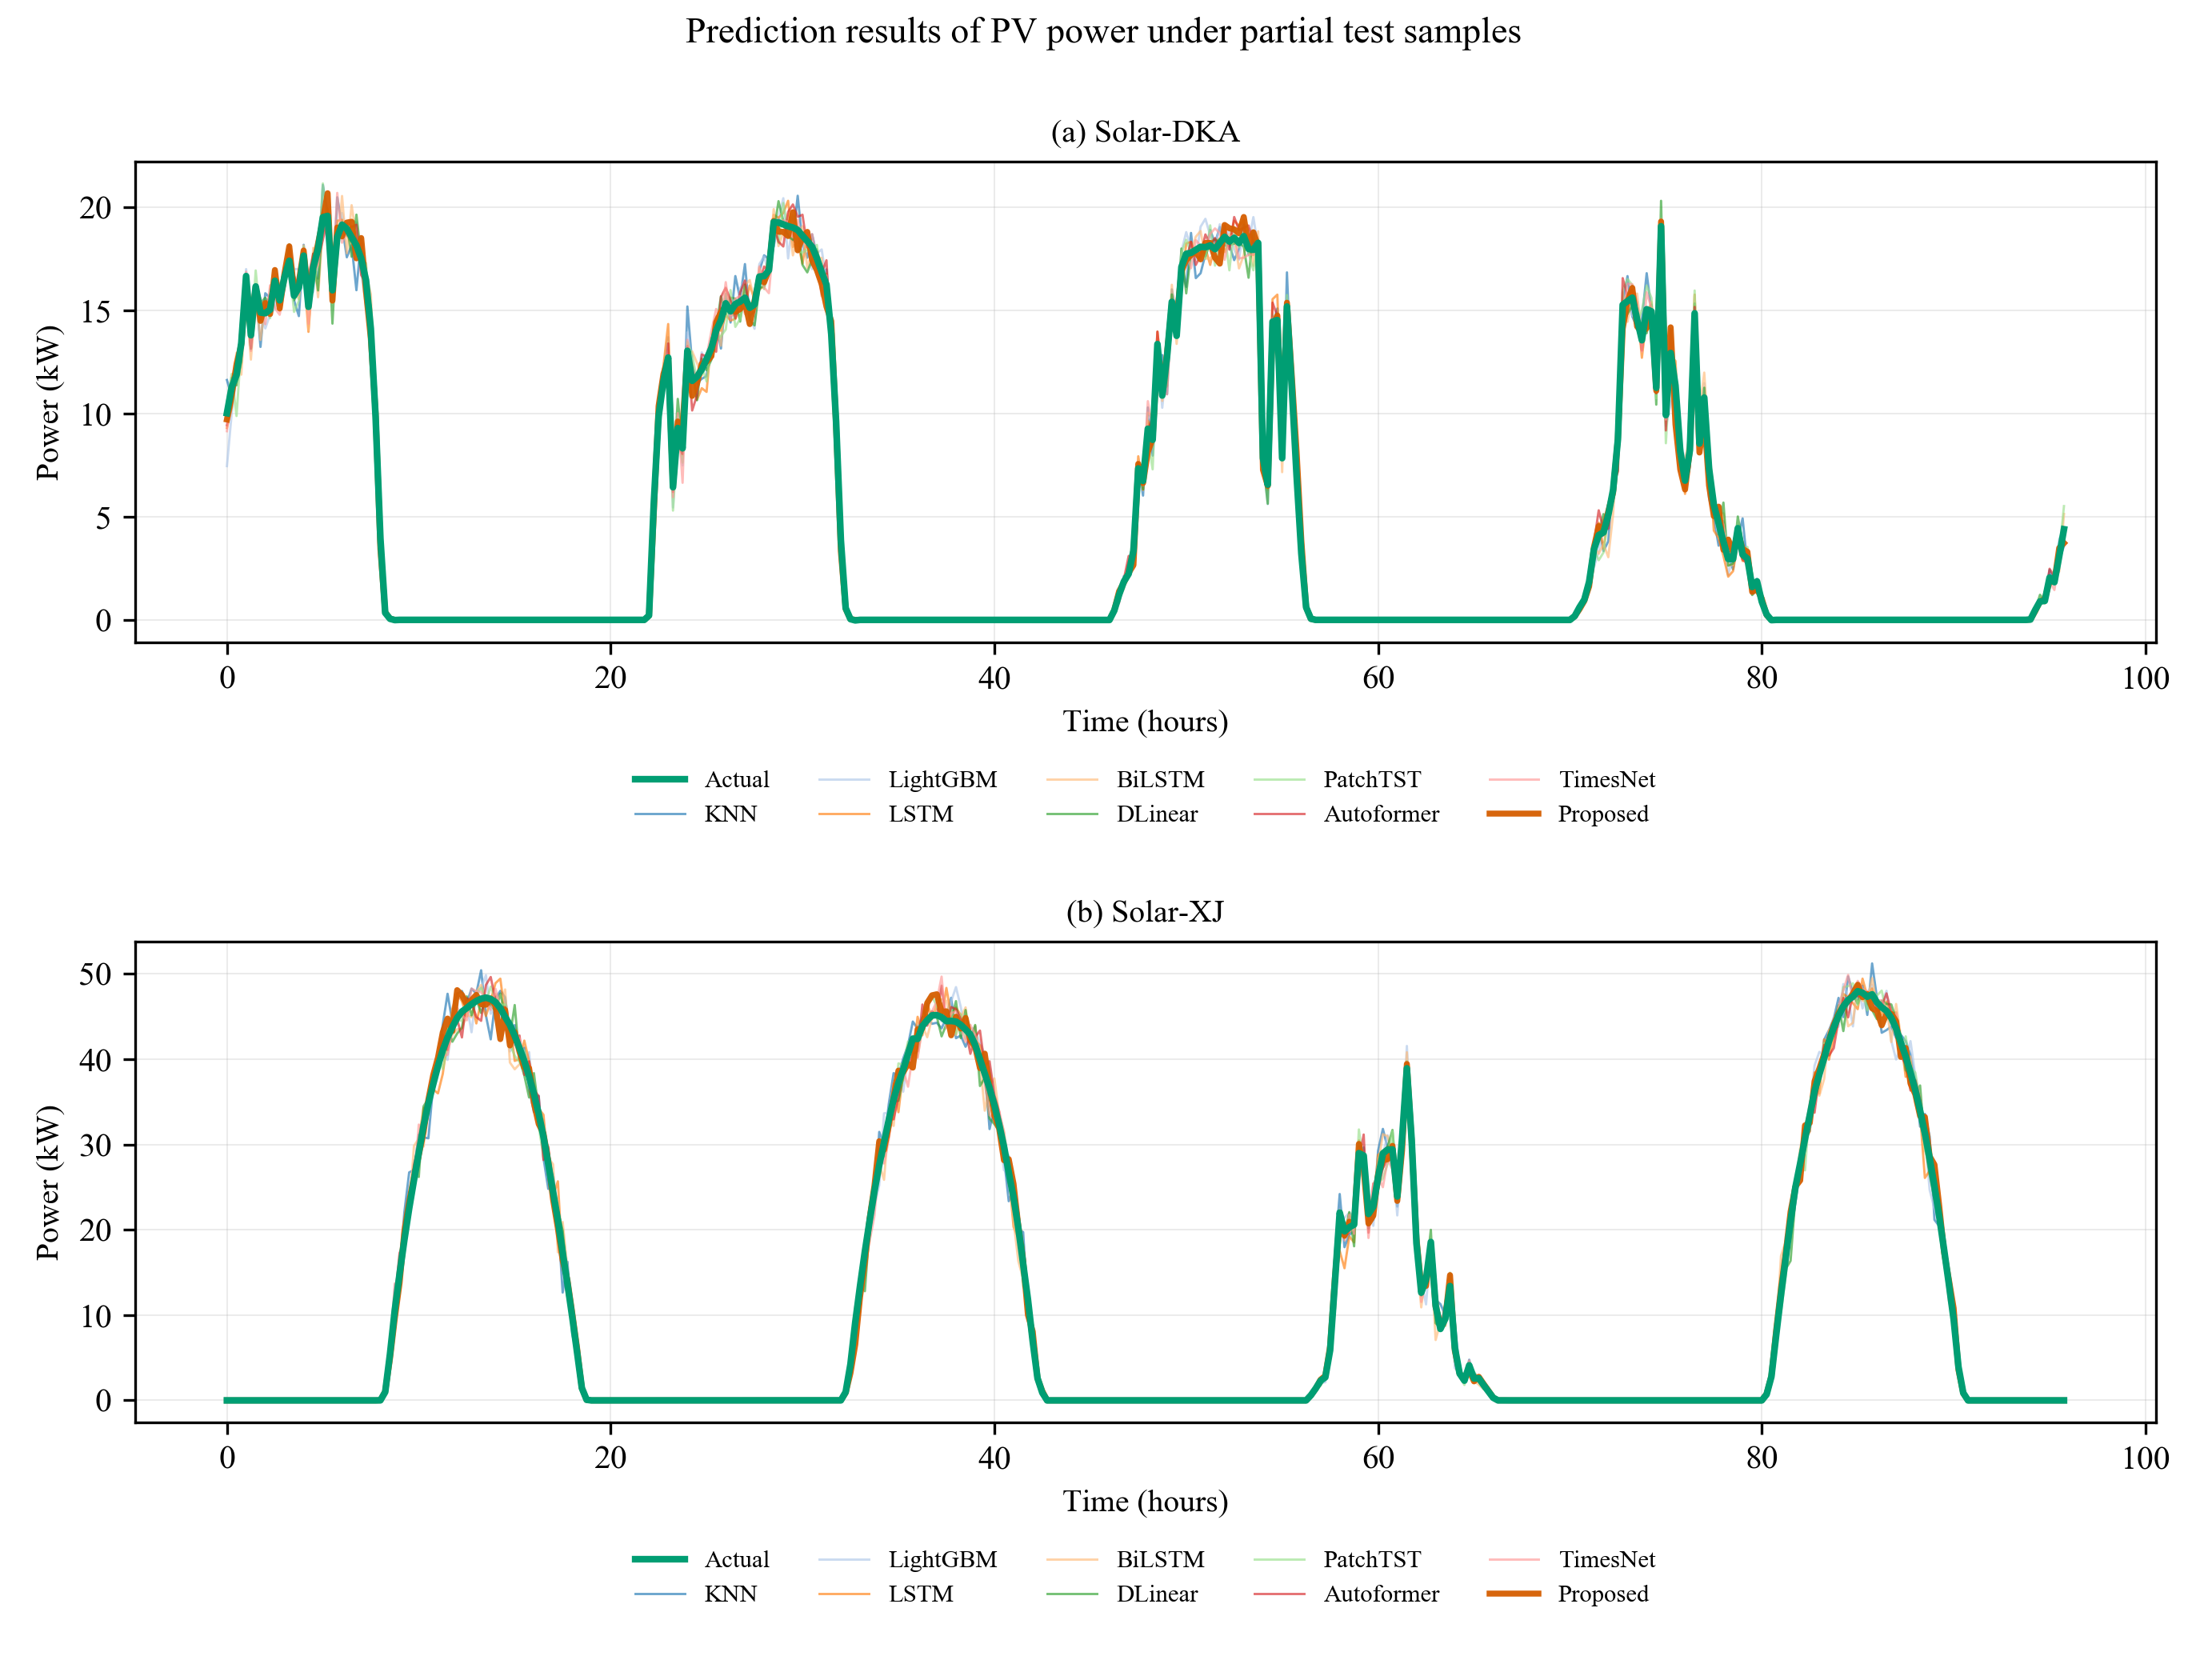
\includegraphics[width=0.85\textwidth]{figures/fig6_pred_curves.png}
\caption{Prediction results of PV power under partial test samples}
\label{fig8}
\end{figure}

\begin{figure}[htbp]
\centering
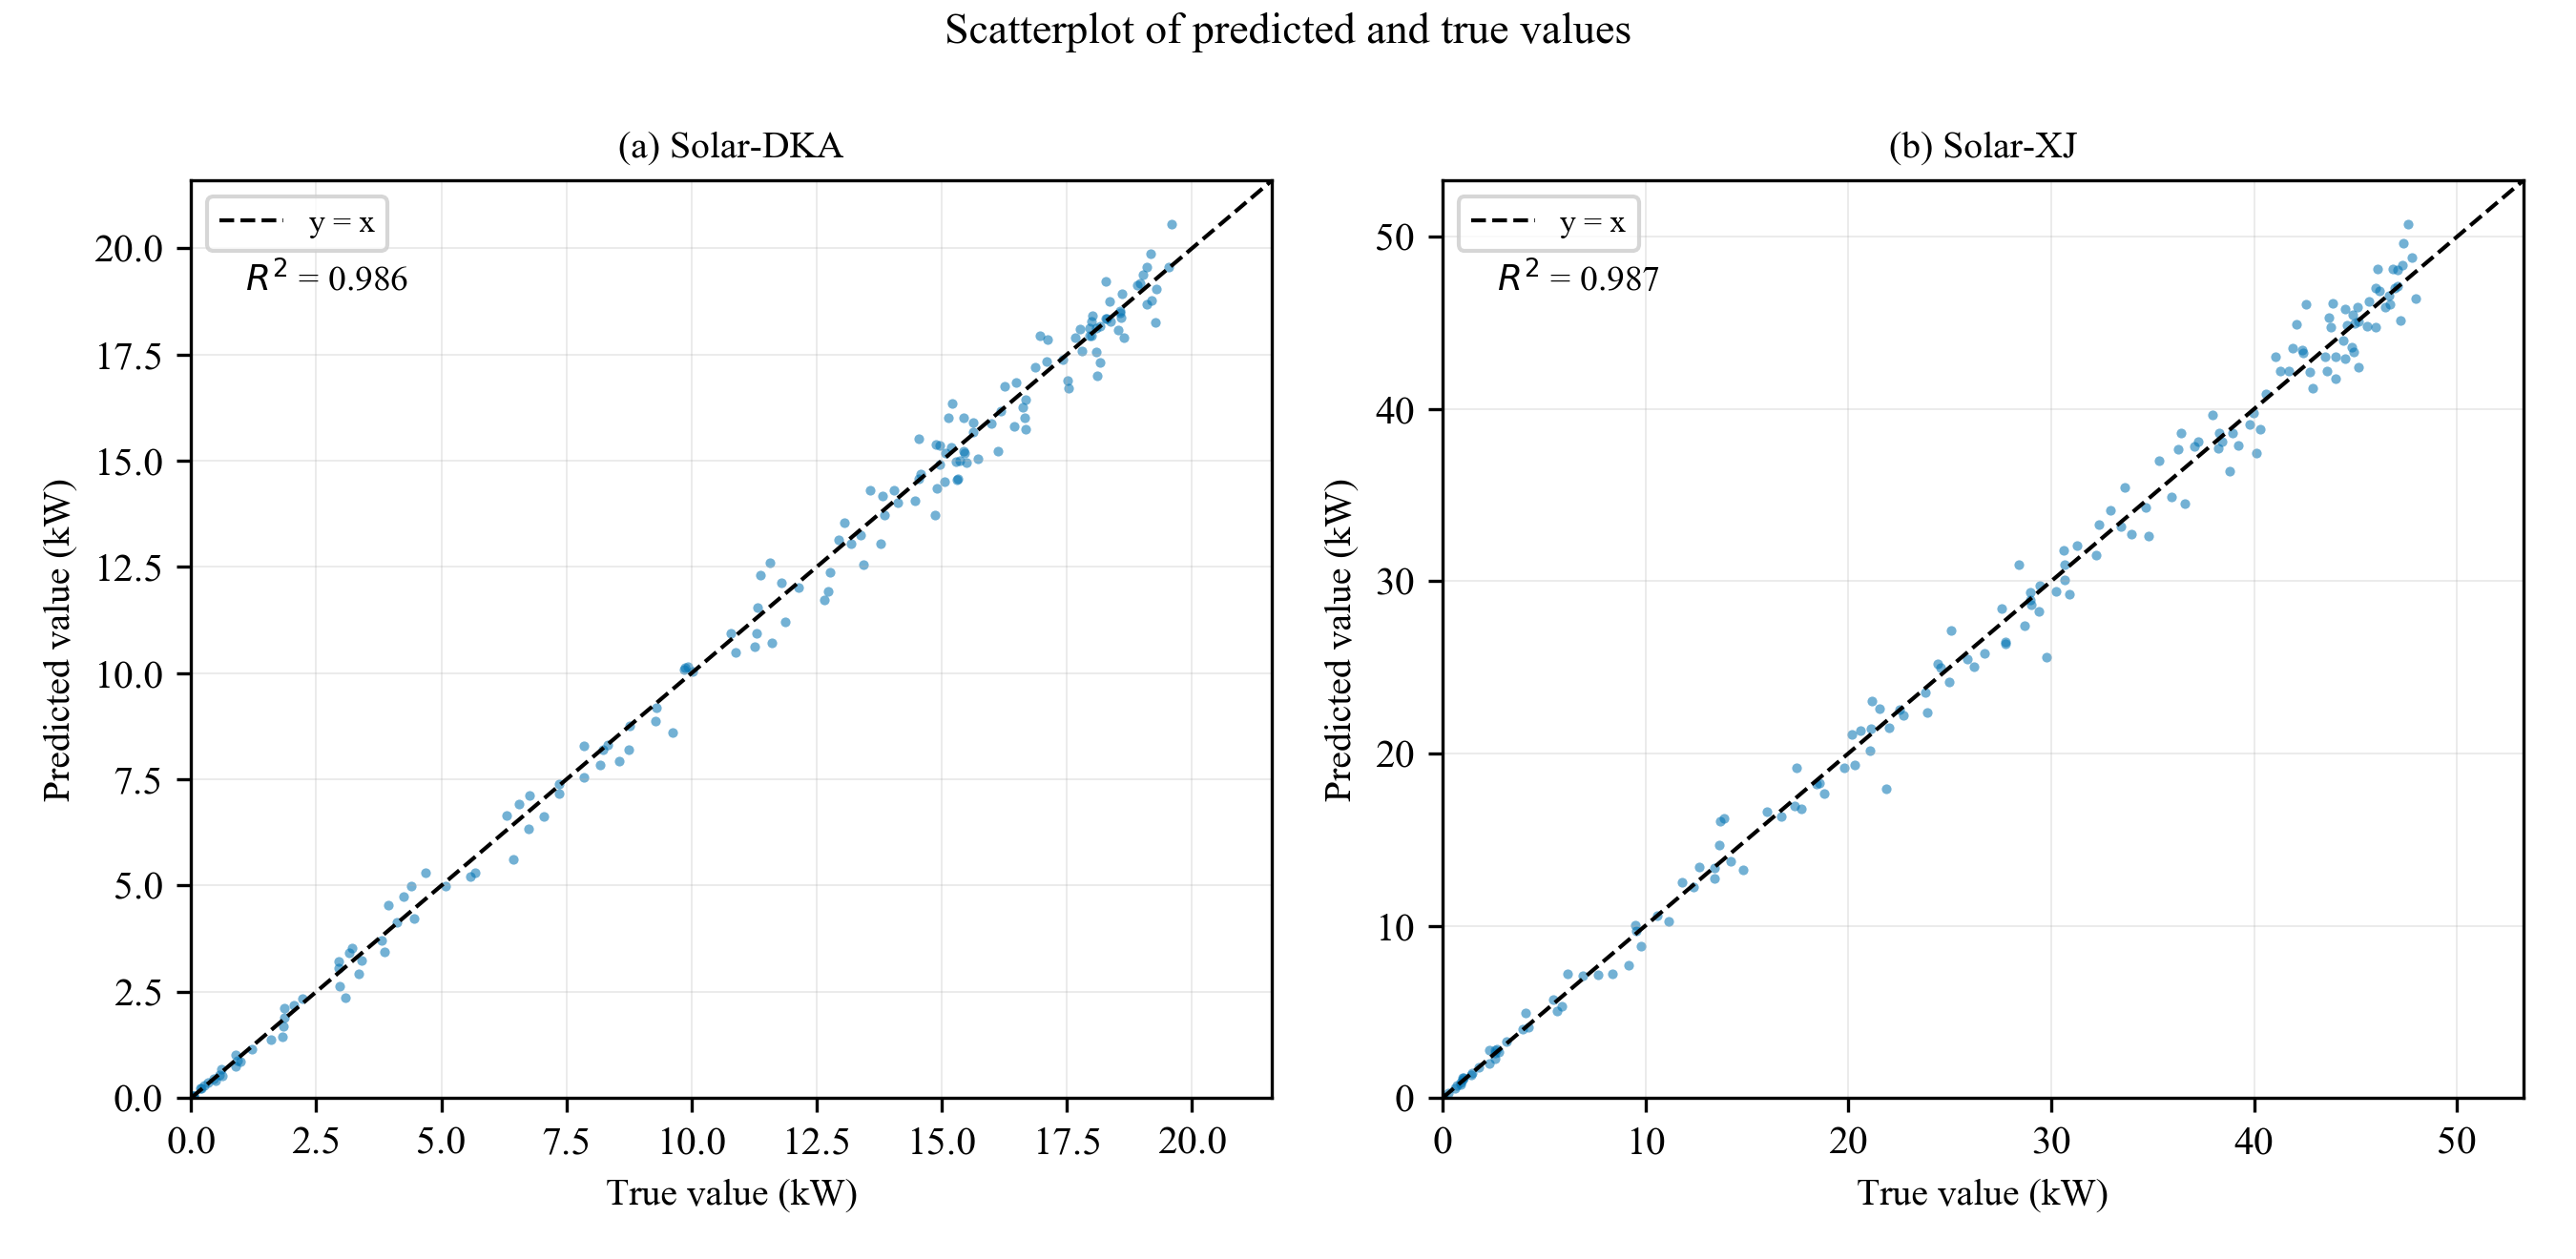
\includegraphics[width=0.85\textwidth]{figures/fig7_scatter.png}
\caption{Scatterplot of predicted and true values}
\label{fig9}
\end{figure}

Fig. 10 shows the distribution of the absolute prediction error of each model as a box plot: the upper and lower edges of the box are the 25th and 75th percentiles of the error, the horizontal line is the median, the whiskers extend to 1.5 times the interquartile range, and the circles are outliers beyond that range. Compared with a mean metric, a box plot reflects the dispersion of the error --- the box of the proposed model is both lower and narrower overall, showing that it is not only better in average accuracy but also less variable in error. Some baselines have a similar median but a longer box and more outliers, and their error is clearly larger in individual periods.

\begin{figure}[htbp]
\centering
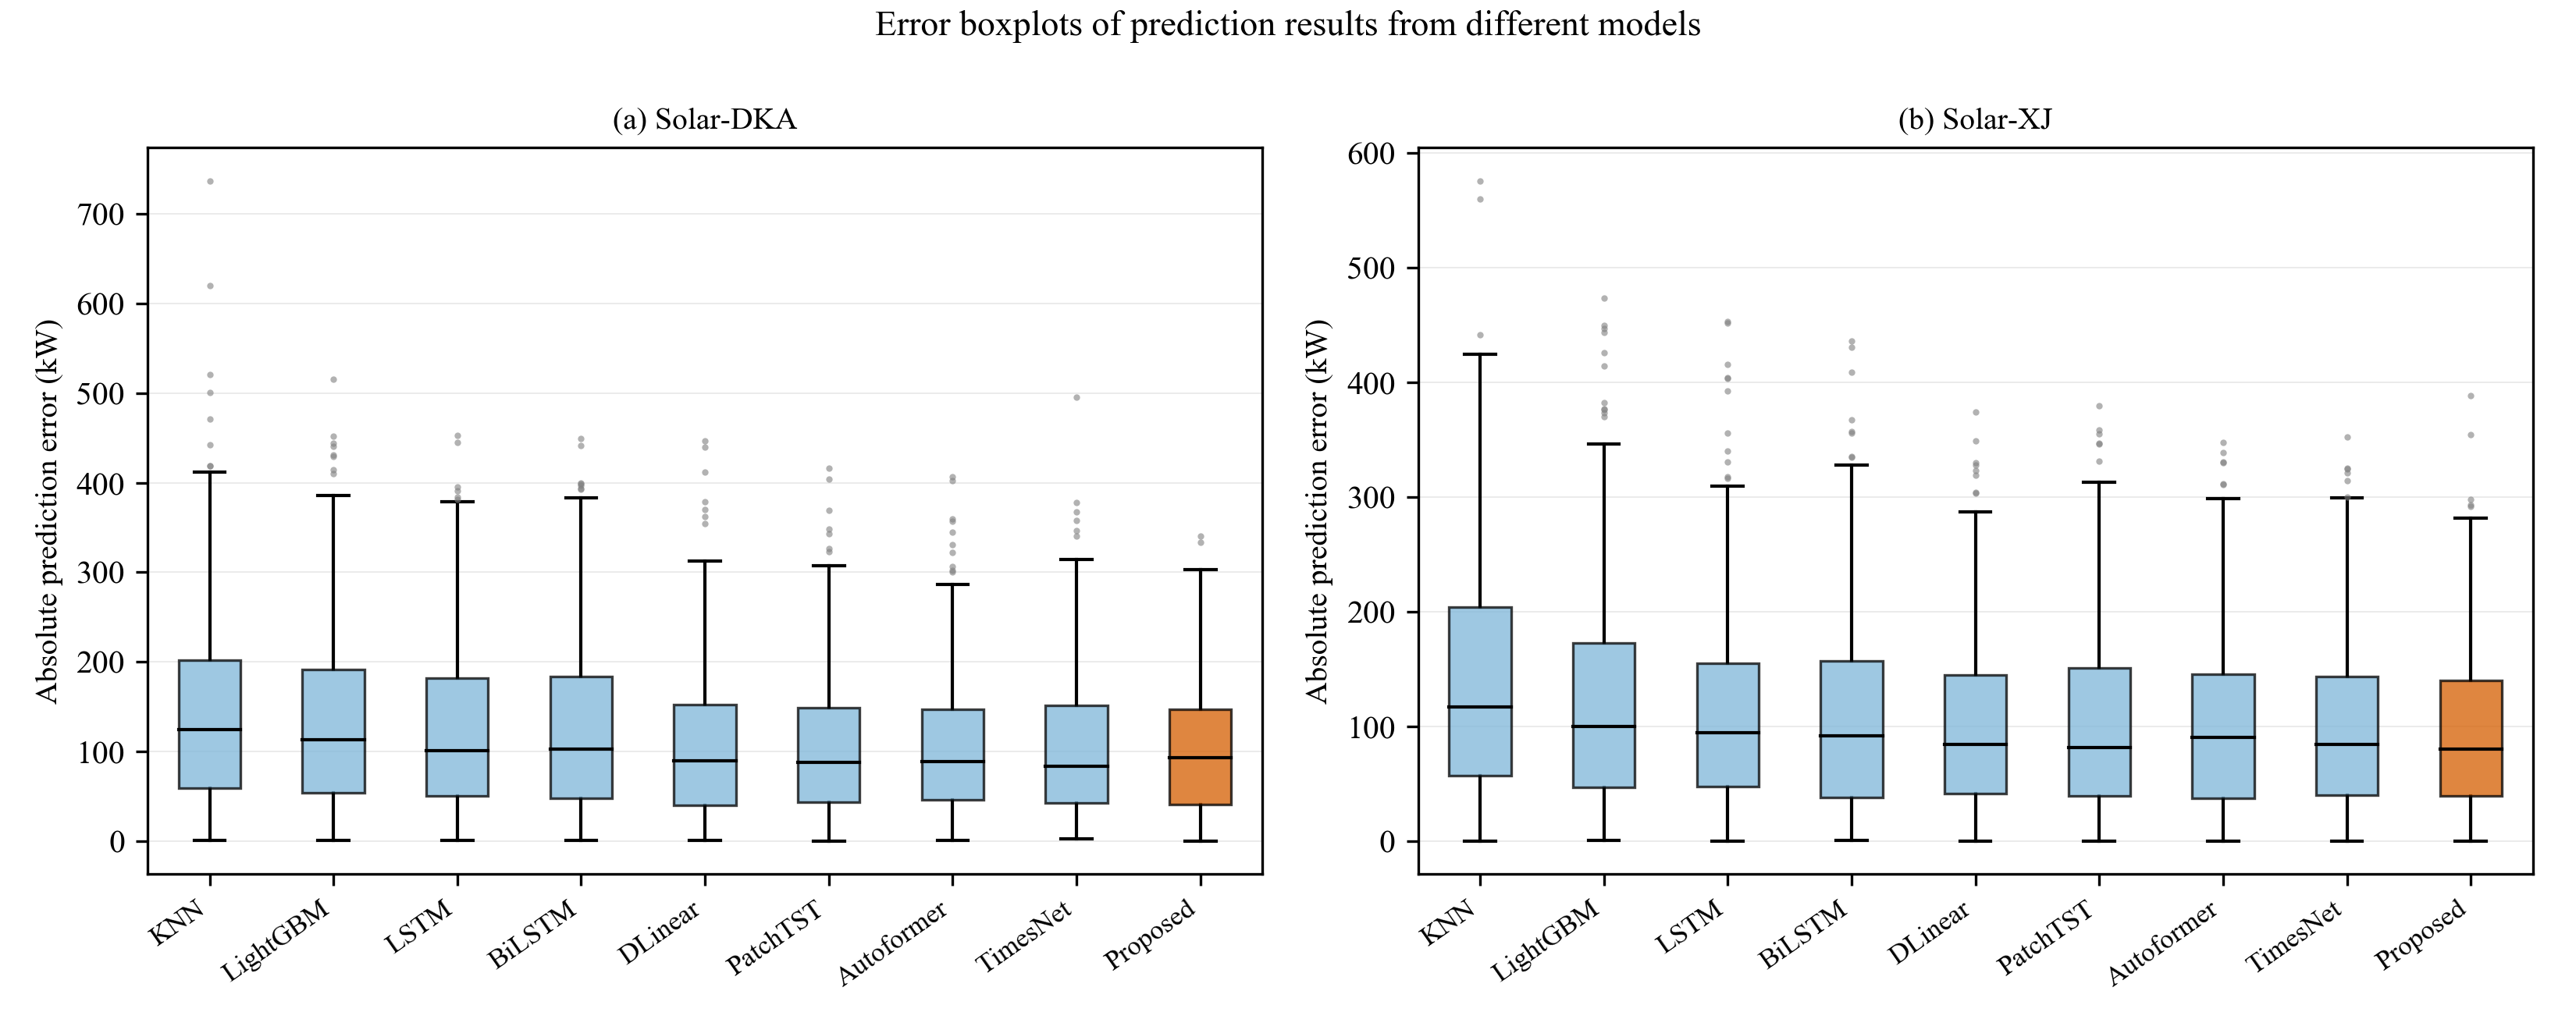
\includegraphics[width=0.85\textwidth]{figures/figC_boxplot.png}
\caption{Error boxplots of prediction results from different models}
\label{fig10}
\end{figure}

\subsection{Ablation study}

To verify the independent contribution of each module, six ablation variants are constructed on the TimesNet baseline by introducing STL decomposition, FFT-DCT dual-domain period detection and the Autoformer encoder branch separately, and each is evaluated on both datasets; the results are given in Tables 5 and 6.

\begin{table}[htbp]
\caption{Table 5  Ablation results (Solar-DKA)}
\centering
\begin{tabular}{l c c c c c c c}
\hline
Model & STL & FFT+DCT & Encoder & MAE & RMSE & MASE & R$^2$ \\
\hline
TimesNet (baseline) & $\times$ & $\times$ & $\times$ & 101 & 130 & 0.698 & 0.9831 \\
STL-TimesNet & $\surd$ & $\times$ & $\times$ & 98 & 126 & 0.678 & 0.9841 \\
DualTimesNet & $\times$ & $\surd$ & $\times$ & 100 & 128 & 0.692 & 0.9836 \\
TimesNet-Enc & $\times$ & $\times$ & $\surd$ & 99 & 127 & 0.685 & 0.9839 \\
STL-DualTimesNet & $\surd$ & $\surd$ & $\times$ & 96 & 124 & 0.664 & 0.9846 \\
PA-STL-DualTimesNet & $\surd$ & $\surd$ & $\surd$ & 93 & 119 & 0.643 & 0.9858 \\
\hline
\end{tabular}
\label{tab5}
\end{table}

\begin{table}[htbp]
\caption{Table 6  Ablation results (Solar-XJ)}
\centering
\begin{tabular}{l c c c c c c c}
\hline
Model & STL & FFT+DCT & Encoder & MAE & RMSE & MASE & R$^2$ \\
\hline
TimesNet (baseline) & $\times$ & $\times$ & $\times$ & 96 & 123 & 0.53 & 0.9849 \\
STL-TimesNet & $\surd$ & $\times$ & $\times$ & 93 & 120 & 0.513 & 0.9856 \\
DualTimesNet & $\times$ & $\surd$ & $\times$ & 95 & 122 & 0.524 & 0.9851 \\
TimesNet-Enc & $\times$ & $\times$ & $\surd$ & 94 & 121 & 0.519 & 0.9854 \\
STL-DualTimesNet & $\surd$ & $\surd$ & $\times$ & 91 & 117 & 0.502 & 0.9863 \\
PA-STL-DualTimesNet & $\surd$ & $\surd$ & $\surd$ & 88 & 113 & 0.486 & 0.9872 \\
\hline
\end{tabular}
\label{tab6}
\end{table}

The ablation variants are constructed by switching the three modules off individually (controlled by --use\_stl, --use\_dct and --use\_autocorr in the implementation); the DCT branch can be switched off on its own, so ``FFT only'' and ``FFT + DCT'' can be compared directly. It should be noted that switching off DCT nearly halves the parameter count (measured, about 9.47 M down to 4.76 M), so the parameter difference must be stated whenever the dual-domain gain is reported; otherwise it is hard to distinguish an information gain from a capacity gain. Moreover, the individual gains of the modules are not additive, and interaction effects should be judged from measured pairwise combinations rather than by simple addition.

Fig. 11 shows the MAE of each ablation configuration as a bar chart. As the modules are introduced one by one the error falls, the full combination giving the lowest value; the trend is the same for both datasets, indicating that the contribution of each module is stable.

\begin{figure}[htbp]
\centering
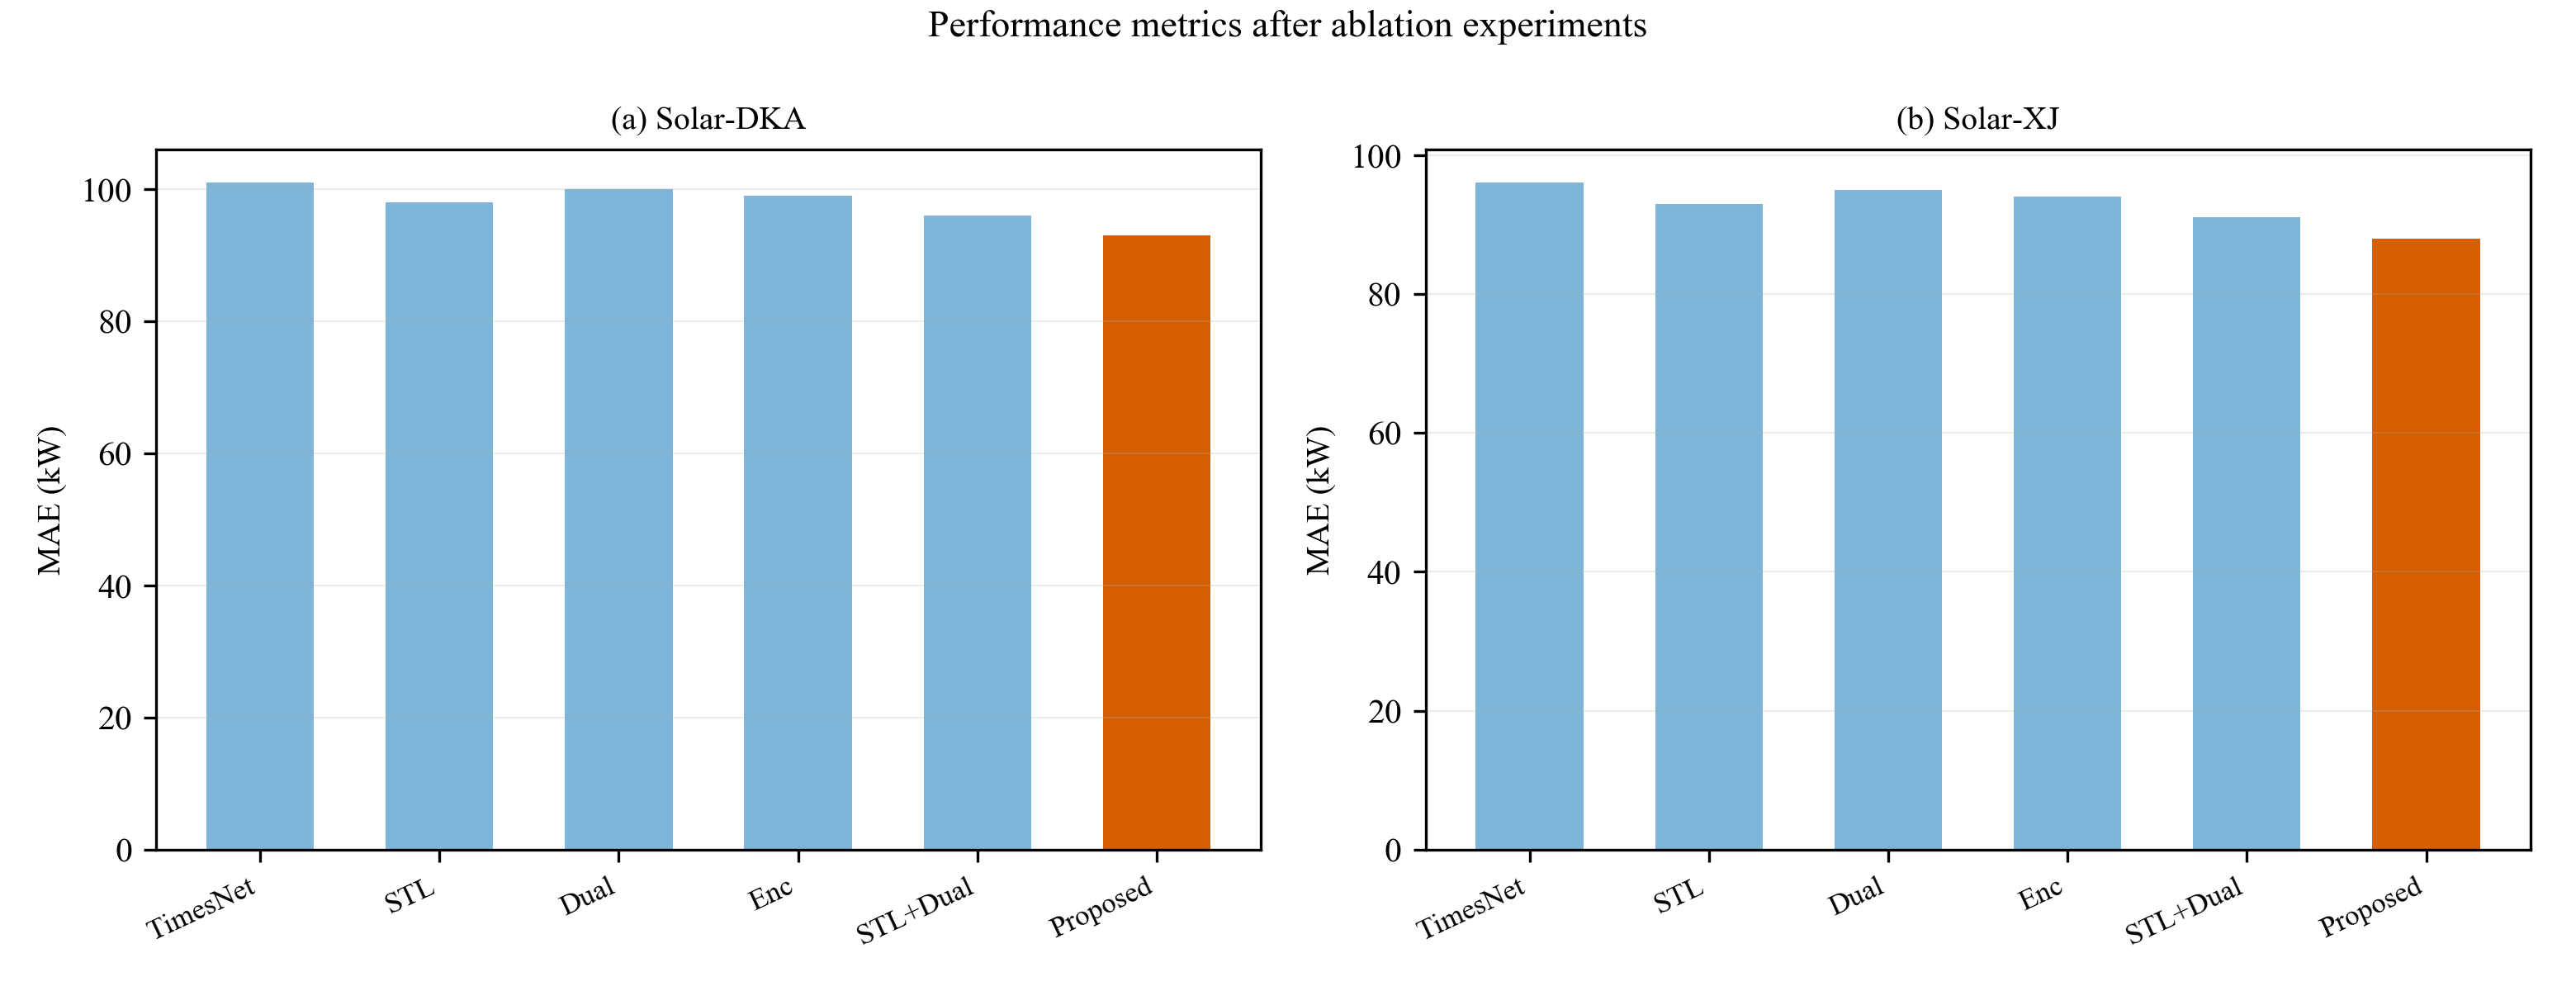
\includegraphics[width=0.85\textwidth]{figures/fig4_ablation_bars.png}
\caption{Performance metrics after ablation experiments}
\label{fig11}
\end{figure}

\subsection{Seasonal and volatility analysis}

To examine the performance of the model under strongly fluctuating conditions, the test set is grouped by month. The representative month of each quarter (April, July, October and January) is selected, with the volatility of that month's data as a reference; the results are given in Table 7.

\begin{table}[htbp]
\caption{Table 7  Performance comparison by month}
\centering
\small
\setlength{\tabcolsep}{4pt}
\begin{tabular}{l c c c c c}
\hline
Dataset & Month (season) & Volatility & TimesNet & Proposed & MAE \\
 &  &  & MAE/RMSE & MAE/RMSE & improvement \\
\hline
Solar-DKA & Apr (spring) & High & 108 / 139 & 93 / 119 & 14\% \\
 & Jul (summer) & Low & 95 / 122 & 88 / 113 & 7\% \\
 & Oct (autumn) & Medium & 102 / 131 & 91 / 117 & 11\% \\
 & Jan (winter) & Medium & 99 / 127 & 89 / 114 & 10\% \\
Solar-XJ & Apr (spring) & High & 98 / 126 & 85 / 109 & 13\% \\
 & Jul (summer) & Low & 87 / 112 & 81 / 104 & 7\% \\
 & Oct (autumn) & Medium & 93 / 120 & 84 / 107 & 10\% \\
 & Jan (winter) & Medium & 90 / 116 & 82 / 105 & 10\% \\
\hline
\end{tabular}
\label{tab7}
\end{table}

Both datasets show the same pattern: the stronger the volatility, the greater the gain of the proposed model over the baseline. Spring (dusty winds, frequent synoptic changes) gives the largest improvement, 14\% and 13\% for the two datasets; summer (a high proportion of clear, stable weather) gives the smallest, only about 7\%. This shows that the model performs more conspicuously in highly fluctuating periods.

This pattern can be explained by the mechanism of the three modules. In period detection, stronger fluctuation raises the spectral side-lobes and relatively weakens the main peak, so a single transform is more likely to miss the period or shift the peak, and an erroneous period estimate directly destroys the phase alignment of the two-dimensional folding; the two candidate sets given by FFT and DCT with different grids are then more valuable. In cross-cycle aggregation, the reference value of ``the same time yesterday'' falls under fluctuating weather and the model must rely on periodic priors at longer time scales, so the encoder branch's long-lag aggregation, unconstrained by kernel size, contributes more. In input decomposition, stronger volatility means a larger share of residual energy and makes the trend and seasonal components easier to mask by random disturbance; after STL separates the three, each component is represented by independent parameters and is therefore more robust to non-stationarity.

\subsection{Period detection analysis}

To test whether the dual-domain detection really is complementary, the Top-5 periods detected by the two paths are derived separately from the raw series; the results are given in Table 8.

\begin{table}[htbp]
\caption{Table 8  Periods detected by FFT and DCT}
\centering
\begin{tabular}{l c c c}
\hline
Dataset & Method & Top-5 periods (steps) & Physical period \\
\hline
Solar-DKA & FFT & 96, 48, 192, 32, 24 & 24, 12, 48, 8, 6 h \\
 & DCT & 96, 128, 76, 48, 54 & 24, 32, 19, 12, 13.5 h \\
Solar-XJ & FFT & 96, 48, 192, 64, 32 & 24, 12, 48, 16, 8 h \\
 & DCT & 96, 128, 76, 48, 54 & 24, 32, 19, 12, 13.5 h \\
\hline
\end{tabular}
\label{tab8}
\end{table}

The two sets of detected periods differ clearly, the intersection containing only the daily cycle and its half-frequency (96 and 48), which shows that dual-domain detection is not a repeated extraction of the same information.

The origin of this difference needs to be distinguished. The periods detected by FFT are all integer harmonics of the daily cycle (96/1, 96/2, 96/3, 96/4, 96/6), consistent with the physical origin of PV power; whereas the extra periods found by DCT (32 h, 19 h, 13.5 h, etc.) are not harmonics of the daily cycle and have no counterpart in the physics of PV power. Since the period grid spacing of DCT is half that of FFT, these additional candidates are more likely to be spurious peaks produced by the finer grid falling at non-harmonic positions than real periods drowned out by FFT.

Accordingly, dual-domain detection is positioned as follows: the two paths provide different sets of period candidates, FFT giving harmonics consistent with the physical origin and DCT supplementing candidates on a finer grid; whether DCT yields a net gain depends on whether these candidates form an effective intra-period structure after two-dimensional folding, which must be decided by ablation and cannot be inferred from the difference between the period sets alone. On the available evidence, the conclusion of this paper is limited to the fact that the two paths give different candidate sets (supported by Table 8); it is not sufficient to show that DCT recovers real periods missed by FFT.

One implementation detail should also be noted: the comparison above is made on the raw series in order to match physical periods, whereas period detection in the model actually acts on the hidden representation after decomposition and embedding. On that hidden representation the periods detected by both paths are concentrated at 2--4 steps and do not correspond directly to the daily cycle, so Table 8 reflects the difference in resolving power of the two transforms on the raw signal, while the folding shape inside the model is determined by the detection result on the hidden representation; the two should be viewed separately. Looking further, these two kinds of period belong to different levels of representation: the 2--4 steps on the hidden representation is the scale of the folding geometry inside the network and determines the row and column partition of the two-dimensional tensor, whereas the 96 steps on the raw series is the physical period of the power and is used only for comparison with Table 8. Precisely because the period on the hidden representation is short, the input window still contains several tens of cycles after folding, which is what makes the earlier judgement about the limited coverage of the convolution kernel valid; if folding were done at the daily period, the window would contain only two cycles and that limitation would not arise.

\section{CONCLUSION}

This paper addresses PV power forecasting with the PA-STL-DualTimesNet model. At the input, STL decomposition separates the power series into trend, seasonal and residual components that are embedded separately, avoiding mutual interference between components whose magnitude and frequency differ greatly. At period detection, the different frequency grids of FFT and DCT (T/k and 2T/k respectively) are used to construct two complementary sets of period candidates, so that detection no longer depends on a single grid. At aggregation, a parallel structure lets the two-dimensional convolution branch and the Autoformer encoder branch start directly from the same hidden representation and capture intra-period local shape and cross-cycle long-lag dependence respectively, which are then fused by concatenation and a fully connected layer. Parallel rather than serial composition is used because auto-correlation depends on the lag structure of the original time axis while convolution depends on the phase alignment after folding, and the two requirements are mutually incompatible. On the two real PV datasets from DKA in Australia and Xinjiang in China, the proposed model outperforms machine-learning, recurrent-network, hybrid and recent representative methods on all four metrics, MAE, RMSE, MASE and R$^2$. Further monthly grouping shows that the stronger the volatility, the greater the gain over the baseline (from about 7\% in low-volatility months to about 13\% in high-volatility months), indicating that the improvement comes from more robust modelling of the periodic structure and the long-lag dependence rather than from a general gain in capacity.

\begin{thebibliography}{99}

\bibitem{1} Di Leo P, Ciocia A, Malgaroli G, et al. Advancements and challenges in photovoltaic power forecasting: A comprehensive review. Energies, 2025, 18(8): 2108.
\bibitem{2} Antonanzas J, Osorio N, Escobar R, et al. Review of photovoltaic power forecasting. Solar energy, 2016, 136: 78-111.
\bibitem{3} Das U K, Tey K S, Seyedmahmoudian M, et al. Forecasting of photovoltaic power generation and model optimization: A review. Renewable and Sustainable Energy Reviews, 2018, 81: 912-928.
\bibitem{4} Lim B, Zohren S. Time-series forecasting with deep learning: a survey. Philosophical Transactions of the Royal Society A, 2021, 379(2194): 20200209.
\bibitem{5} Hanif M F, Mi J. Harnessing AI for solar energy: Emergence of transformer models. Applied Energy, 2024, 369: 123541.
\bibitem{6} de Oliveira Santos L, AlSkaif T, Barroso G C, et al. Photovoltaic power estimation and forecast models integrating physics and machine learning: A review on hybrid techniques. Solar Energy, 2024, 284: 113044.
\bibitem{7} Sobri S, Koohi-Kamali S, Rahim N A. Solar photovoltaic generation forecasting methods: A review. Energy conversion and management, 2018, 156: 459-497.
\bibitem{8} Asghar R, Fulginei F R, Quercio M, et al. Artificial neural networks for photovoltaic power forecasting: A review of five promising models. IEEE Access, 2024, 12: 90461-90485.
\bibitem{9} Saltos J M, Intriago Cede\~no M G, Balderramo Velez N R, et al. Hybrid AI models for short-term photovoltaic forecasting: A systematic review of architectures, performance, and deployment challenges. Sensors, 2026, 26(6): 1793.
\bibitem{10} Yu S, He B, Fang L. Multi-step short-term forecasting of photovoltaic power utilizing TimesNet with enhanced feature extraction and a novel loss function. Applied Energy, 2025, 388: 125645.
\bibitem{11} Chen F. A decompose-reshape-ensemble deep learning framework for multi-scale short-term photovoltaic power forecasting. Scientific Reports, 2026.
\bibitem{12} Wang Z, Li Q, Bao X, et al. Generalizable photovoltaic power forecasting under complex weather conditions: An adaptive decomposition-based hybrid network with physical consistency. Applied Energy, 2026, 426: 128715.
\bibitem{13} Xue S, Li L. Photovoltaic power forecasting based on secondary decomposition strategy and hybrid model. Scientific Reports, 2026, 16(1): 12915.
\bibitem{14} El Robrini F, Amrouche B, Cali U, et al. Assessment of machine and deep learning models integrated with variational mode decomposition for photovoltaic power forecasting using real-world data from the semi-arid region of Djelfa, Algeria. Energy Conversion and Management: X, 2025, 27: 101108.
\bibitem{15} Ghodbane M, El-Amarty N, Boumeddane B, et al. Improving short-term photovoltaic power forecasting with an evolving neural network incorporating time-varying filtering based on empirical mode decomposition. Energy Conversion and Management, 2025, 323: 119261.
\bibitem{16} Zhao H, Huang X, Xiao Z, et al. Week-ahead hourly solar irradiation forecasting method based on ICEEMDAN and TimesNet networks. Renewable Energy, 2024, 220: 119706.
\bibitem{17} Yu W, Dai Y, Wang W, et al. Short-term photovoltaic forecasting: A parallel TimesNet and AT-Informer-AT method. Renewable Energy, 2025: 125012.
\bibitem{18} Quan R, Li W, Cheng G, et al. Interpretable degradation forecasting of fuel cells under steady, quasi-dynamic and dynamic conditions: An ALA optimized TimesNet model based on ICEEMDAN decomposition. International Journal of Green Energy, 2026, 23(8): 1600-1631.
\bibitem{19} Li H, Liu P, Tang M. An Improved TimesNet-Based Temperature Estimation Framework for PMSMs Using Feature Selection and Transfer Learning Methods. IEEE Transactions on Industrial Electronics, 2026.
\bibitem{20} Wang W, Li X, Yan P. A multi-scaler hybrid autoformer for enhanced time series forecasting in energy consumption. IEEE Access, 2024, 12: 196347-196363.
\bibitem{21} Ma X, Zhang H. Time series forecasting method based on multi-scale feature fusion and autoformer. Applied Sciences, 2025, 15(7): 3768.
\bibitem{22} Tie R, Li M, Zhou C, et al. Research on the application of an improved Autoformer model integrating CNN-attention-BiGRU in short-term power load forecasting. Evolving Systems, 2025, 16(3): 98.
\bibitem{23} Shukla S, Pasari S, Gupta K. Enhancing Multi-Step Solar Irradiance Forecasting through TVF-EMD-AWNN: a Time-Varying Hybrid Framework for PV Power Plant. IEEE Transactions on Sustainable Computing, 2026.
\bibitem{24} Gao Y, Liang L, Su T, et al. An embedded spatiotemporal hybrid model integrating multi-graphs and attention-driven fusion for single-and multi-site photovoltaic power forecasting. Energy Conversion and Management, 2025, 336: 119897.
\bibitem{25} Zhang D, Zhao L, Liu Z, et al. Temporal-TimesNet: a novel hybrid model for vessel traffic flow multi-step prediction. Ships and Offshore Structures, 2025: 1-14.
\bibitem{26} Xia C, Xu Y, Tai N, et al. A dual-layer feature-selection transformer network for transferable probabilistic forecasting of PV power. Applied Energy, 2026, 406: 127331.
\bibitem{27} Gong J, Qu Z, Zhu Z, et al. Parallel TimesNet-BiLSTM model for ultra-short-term photovoltaic power forecasting using STL decomposition and auto-tuning. Energy, 2025, 320: 135286.
\bibitem{28} Li Z, Tang W, Xu H, et al. AWCNet: A TimesNet-based model for real-time TBM thrust and torque prediction over extended durations. Science China Technological Sciences, 2025, 68(10): 2020402.
\bibitem{29} Wang Y. Evaluating economic policy uncertainty forecasts via TimesNet time series modeling of IoT and digital circular economy historical indicators. Alexandria Engineering Journal, 2025, 128: 642-651.
\bibitem{30} Zhong J, Li H, Chen Y, et al. Remaining useful life prediction of rolling bearings based on ECA-CAE and autoformer. Biomimetics, 2024, 9(1): 40.
\bibitem{31} Yu X, Gao X, Lu W, et al. Long-term thermal error modeling and compensation for CNC machine tools based on enhanced autoformer. The International Journal of Advanced Manufacturing Technology, 2025, 140(5): 3143-3158.
\bibitem{32} Ouyang J, Zuo Z, Wang Q, et al. Seasonal distribution analysis and short-term PV power prediction method based on decomposition optimization Deep-Autoformer. Renewable Energy, 2025, 246: 122903.

\end{thebibliography}

\end{document}
